% This is samplepaper.tex, a sample chapter demonstrating the
% LLNCS macro package for Springer Computer Science proceedings;
% Version 2.20 of 2017/10/04
%
%\documentclass[runningheads]{report}
\documentclass{article}
%
\usepackage{graphicx}
\usepackage{comment}
\usepackage{indentfirst}
\usepackage{float}
% Used for displaying a sample figure. If possible, figure files should
% be included in EPS format.
%
% If you use the hyperref package, please uncomment the following line
% to display URLs in blue roman font according to Springer's eBook style:
% \renewcommand\UrlFont{\color{blue}\rmfamily}

\begin{document}
%
\title{ECE219 Project 3\\ Collaborative Filtering}
%
%\titlerunning{Abbreviated paper title}
% If the paper title is too long for the running head, you can set
% an abbreviated paper title here
%
\author{Zhilai~Shen, Yufei~Hu, Zheang~Huai, and Tianyi~Liu \\
105023454, 404944367, 505222324, 705035425
}
%
% First names are abbreviated in the running head.
% If there are more than two authors, 'et al.' is used.
%              % typeset the header of the contribution

%
%
%
%
\begin{comment}
\section{First Section}
\subsection{A Subsection Sample}
Please note that the first paragraph of a section or subsection is
not indented. The first paragraph that follows a table, figure,
equation etc. does not need an indent, either.

Subsequent paragraphs, however, are indented.

\subsubsection{Sample Heading (Third Level)} Only two levels of
headings should be numbered. Lower level headings remain unnumbered;
they are formatted as run-in headings.

\paragraph{Sample Heading (Fourth Level)}
The contribution should contain no more than four levels of
headings. Table~\ref{tab1} gives a summary of all heading levels.

\begin{table}
\caption{Table captions should be placed above the
tables.}\label{tab1}
\begin{tabular}{|l|l|l|}
\hline
Heading level &  Example & Font size and style\\
\hline
Title (centered) &  {\Large\bfseries Lecture Notes} & 14 point, bold\\
1st-level heading &  {\large\bfseries 1 Introduction} & 12 point, bold\\
2nd-level heading & {\bfseries 2.1 Printing Area} & 10 point, bold\\
3rd-level heading & {\bfseries Run-in Heading in Bold.} Text follows & 10 point, bold\\
4th-level heading & {\itshape Lowest Level Heading.} Text follows & 10 point, italic\\
\hline
\end{tabular}
\end{table}


\noindent Displayed equations are centered and set on a separate
line.
\begin{equation}
x + y = z
\end{equation}
Please try to avoid rasterized images for line-art diagrams and
schemas. Whenever possible, use vector graphics instead (see
Fig.~\ref{fig1}).

\begin{figure}[!htbp]
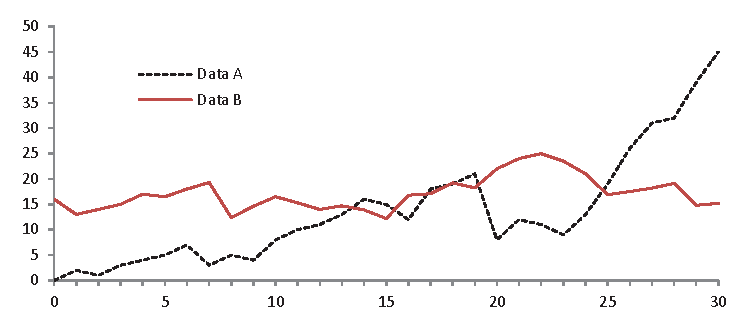
\includegraphics[width=\textwidth]{Figure/fig1.eps}
\caption{A figure caption is always placed below the illustration.
Please note that short captions are centered, while long ones are
justified by the macro package automatically.} \label{fig1}
\end{figure}

\begin{theorem}
This is a sample theorem. The run-in heading is set in bold, while
the following text appears in italics. Definitions, lemmas,
propositions, and corollaries are styled the same way.
\end{theorem}
%
% the environments 'definition', 'lemma', 'proposition', 'corollary',
% 'remark', and 'example' are defined in the LLNCS documentclass as well.
%
\begin{proof}
Proofs, examples, and remarks have the initial word in italics,
while the following text appears in normal font.
\end{proof}
For citations of references, we prefer the use of square brackets
and consecutive numbers. Citations using labels or the author/year
convention are also acceptable. The following bibliography provides
a sample reference list with entries for journal
articles~\cite{ref_article1}, an LNCS chapter~\cite{ref_lncs1}, a
book~\cite{ref_book1}, proceedings without editors~\cite{ref_proc1},
and a homepage~\cite{ref_url1}. Multiple citations are grouped
\cite{ref_article1,ref_lncs1,ref_book1},
\cite{ref_article1,ref_book1,ref_proc1,ref_url1}.
%
% ---- Bibliography ----
%
% BibTeX users should specify bibliography style 'splncs04'.
% References will then be sorted and formatted in the correct style.
%
% \bibliographystyle{splncs04}
% \bibliography{mybibliography}
%

\end{comment}

\begin{titlepage}
	\centering
	\includegraphics[width=0.15\textwidth]{UCLA.png}\par\vspace{1cm}
	\vspace{1cm}
	{\scshape\Large ECE219 Project 4 \par}
	\vspace{1.5cm}
	{\huge\bfseries Regression Analysis\par}
	\vspace{2cm}
	{\Large\itshape Zhilai~Shen, Yufei~Hu, Zheang~Huai, and Tianyi~Liu\par}
	{\Large\itshape 105023454, 404944367, 505222324, 705035425\par}
	\vfill

	\vfill

% Bottom of the page
	{\large \today\par}
\end{titlepage}

\tableofcontents

\newpage

\section{Network Backup Dataset}

\subsection{Load the dataset}
(a) The plot is as in figure \ref{1a}:

\begin{figure}[!htbp]
\centering
\scalebox{0.2}{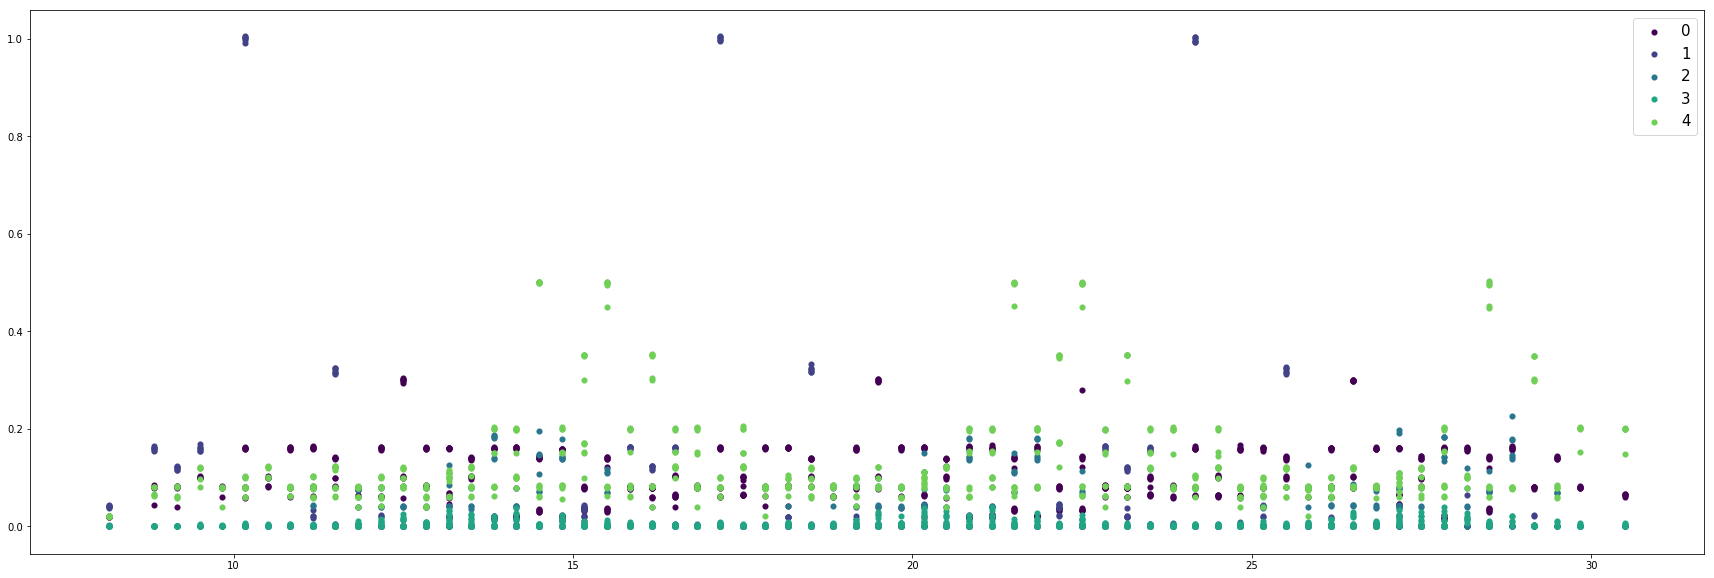
\includegraphics{Figure/1a.png}}
\caption{20 days time vs 20 days backup size} \label{1a}
\end{figure}

(b)The plot is as in figure \ref{1b}:


\begin{figure}[!htbp]
\centering
\scalebox{0.2}{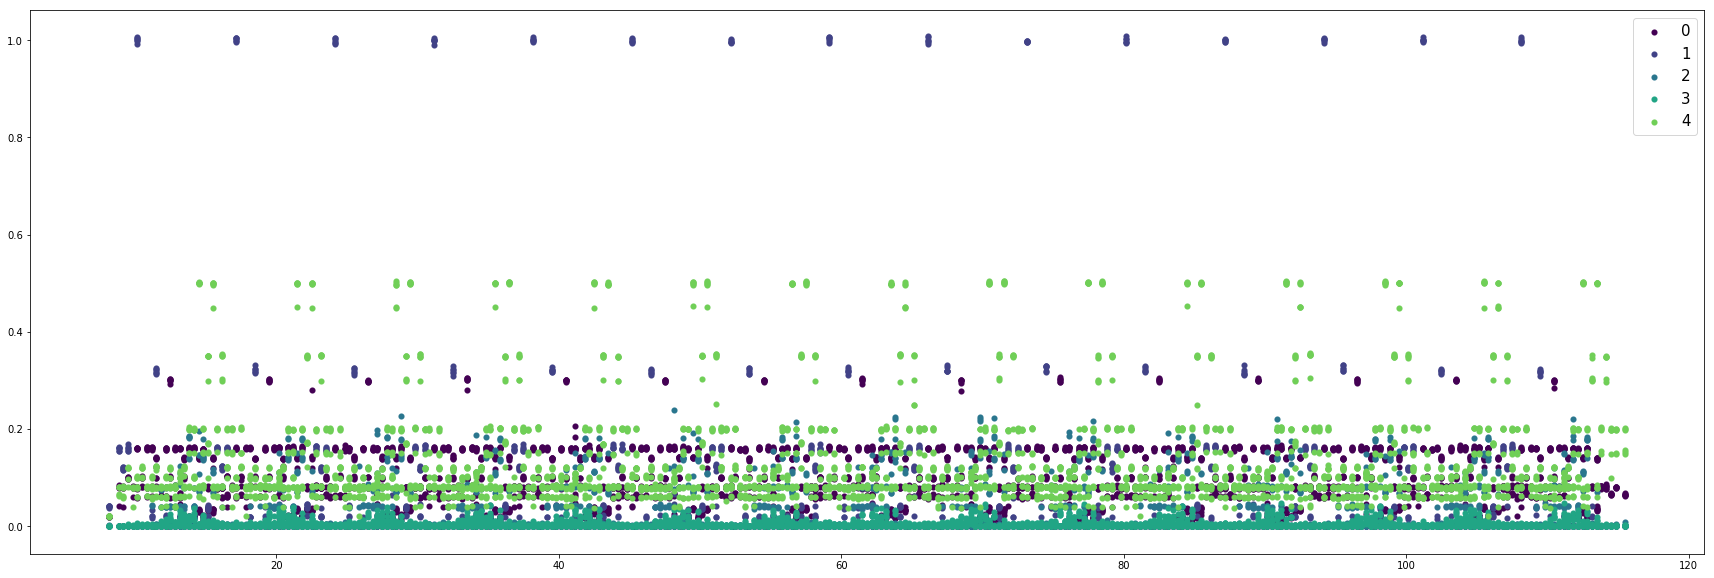
\includegraphics{Figure/1b.png}}
\caption{105 days time vs 105 days backup size} \label{1b}
\end{figure}

(c)As shown in the above graphs, there are in fact repeating patterns. For a constant period of time, work-flow1 will upload a file with size around 1GB. Work-flow3 barely made any backup. Work-flow 0 is constantly used to backup some small files with size around 0.2GB. 

\subsection{Predict the backup size of a file given the other attributes}

\subsubsection{linear regression model}
Fit the linear regression model. \\
All the data are converted into one-dimension. The RMSE for training across ten sets is $0.10358719585332854$, and RMSE for testing across ten sets is $0.10358269769007267$. The fitted value against true value is in figure \ref{2ai}, and the residuals vs fitted values is in figure \ref{2aii}. \\

\begin{figure}[!htbp]
\centering
\scalebox{0.7}{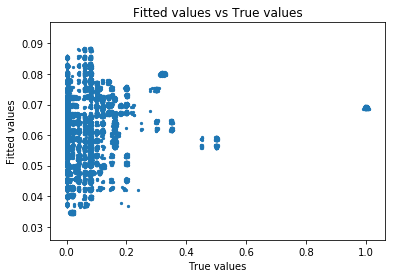
\includegraphics{Figure/2ai.png}}
\caption{Fitted Value vs True Value} \label{2ai}
\end{figure}

\begin{figure}[!htbp]
\centering
\scalebox{0.7}{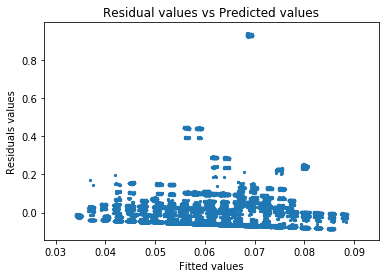
\includegraphics{Figure/2aii.png}}
\caption{Residual vs Fitted Value} \label{2aii}
\end{figure}

\subsubsection{random forest regression model}

Fit the random forest tree model.\\

(i)For the initial model, the RMSE for training is $0.06041914907193139$, and the average RMSE for testing is $0.06077076528311328$. The average out of bag error is $0.3411795413509088$.\\

(ii)After sweeping the maximum number of trees from 1 to 200, and maximum number of features from 1 to 5 and applying the cross-validation using 10 fold, the plot for out of bag error vs number of trees is in figure \ref{2bii1}, and the plot for average test-RMSE vs number of trees is in figure \ref{2bii2}.\\

\begin{figure}[!htbp]
\centering
\scalebox{0.7}{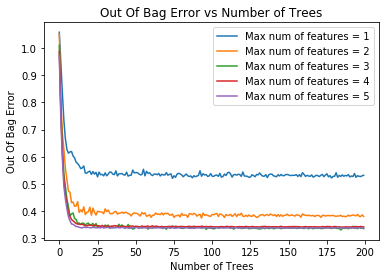
\includegraphics{Figure/2bii1.png}}
\caption{Out of bag error vs number of trees} \label{2bii1}
\end{figure}

\begin{figure}[!htbp]
\centering
\scalebox{0.7}{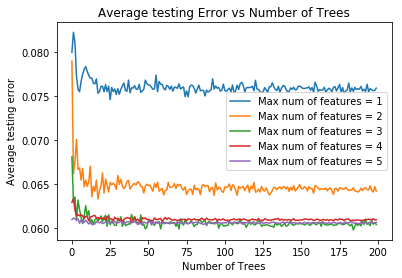
\includegraphics{Figure/2bii2.png}}
\caption{Average test-RMSE vs number of trees} \label{2bii2}
\end{figure}

(iii)For further test, the number of maximum depth is chosen. The depth of each tree is swept from 1 to 30 to find a good performance. The plot for out of bag error vs number of trees is in figure \ref{2biii1}, and the plot for average test-RMSE vs number of trees is in figure \ref{2biii2}. As seen from plots in part (ii) and part (iii), the best hyperparameter is to use maximum number of features = 3, maximum number of trees = 25, and maximum depth = 7.\\

\begin{figure}[!htbp]
\centering
\scalebox{0.7}{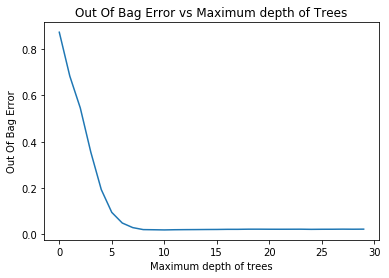
\includegraphics{Figure/2biii1.png}}
\caption{Out of bag error vs number of trees} \label{2biii1}
\end{figure}

\begin{figure}[!htbp]
\centering
\scalebox{0.7}{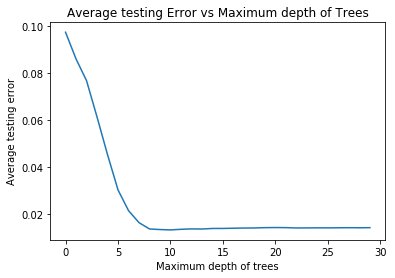
\includegraphics{Figure/2biii2.png}}
\caption{Average test-RMSE vs number of trees} \label{2biii2}
\end{figure}

(iv)The feature importance for the best model in part (iii) is in table \ref{tab:2biv}. 

\begin{table}[h]
\center
\caption{Feature Importance}
\scalebox{0.9}{
\begin{tabular}{c|c}
\hline
Feature Name & Importance \\\hline
Day of the Week & 0.28760693 \\\hline
Hour of the Day & 0.3216406 \\\hline
Work-flow-ID & 0.20244174 \\\hline
File Name & 0.18558651\\\hline
Week Number & 0.00272422\\\hline
\end{tabular}}
\label{tab:2biv}
\end{table}

The average RMSE for training is $0.021061323772690425$, and the average RMSE for testing is $0.021657162672114462$. The fitted value against true value is in figure \ref{2biv1}, and the residuals vs fitted values is in figure \ref{2biv2}. \\

\begin{figure}[!htbp]
\centering
\scalebox{0.7}{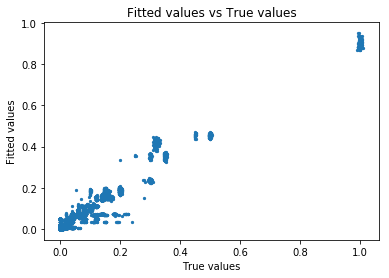
\includegraphics{Figure/2biv1.png}}
\caption{Fitted Value vs True Value} \label{2biv1}
\end{figure}

\begin{figure}[!htbp]
\centering
\scalebox{0.7}{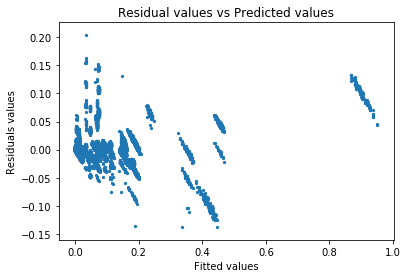
\includegraphics{Figure/2biv2.png}}
\caption{Residual vs Fitted Value} \label{2biv2}
\end{figure} 

(v)The decision tree is in figure \ref{2bv}. The tree node is work-flow-id, which is not the most important feature but a relatively important feature according to the feature importance in part (iv). 

\begin{figure}[!htbp]
\centering
\scalebox{0.15}{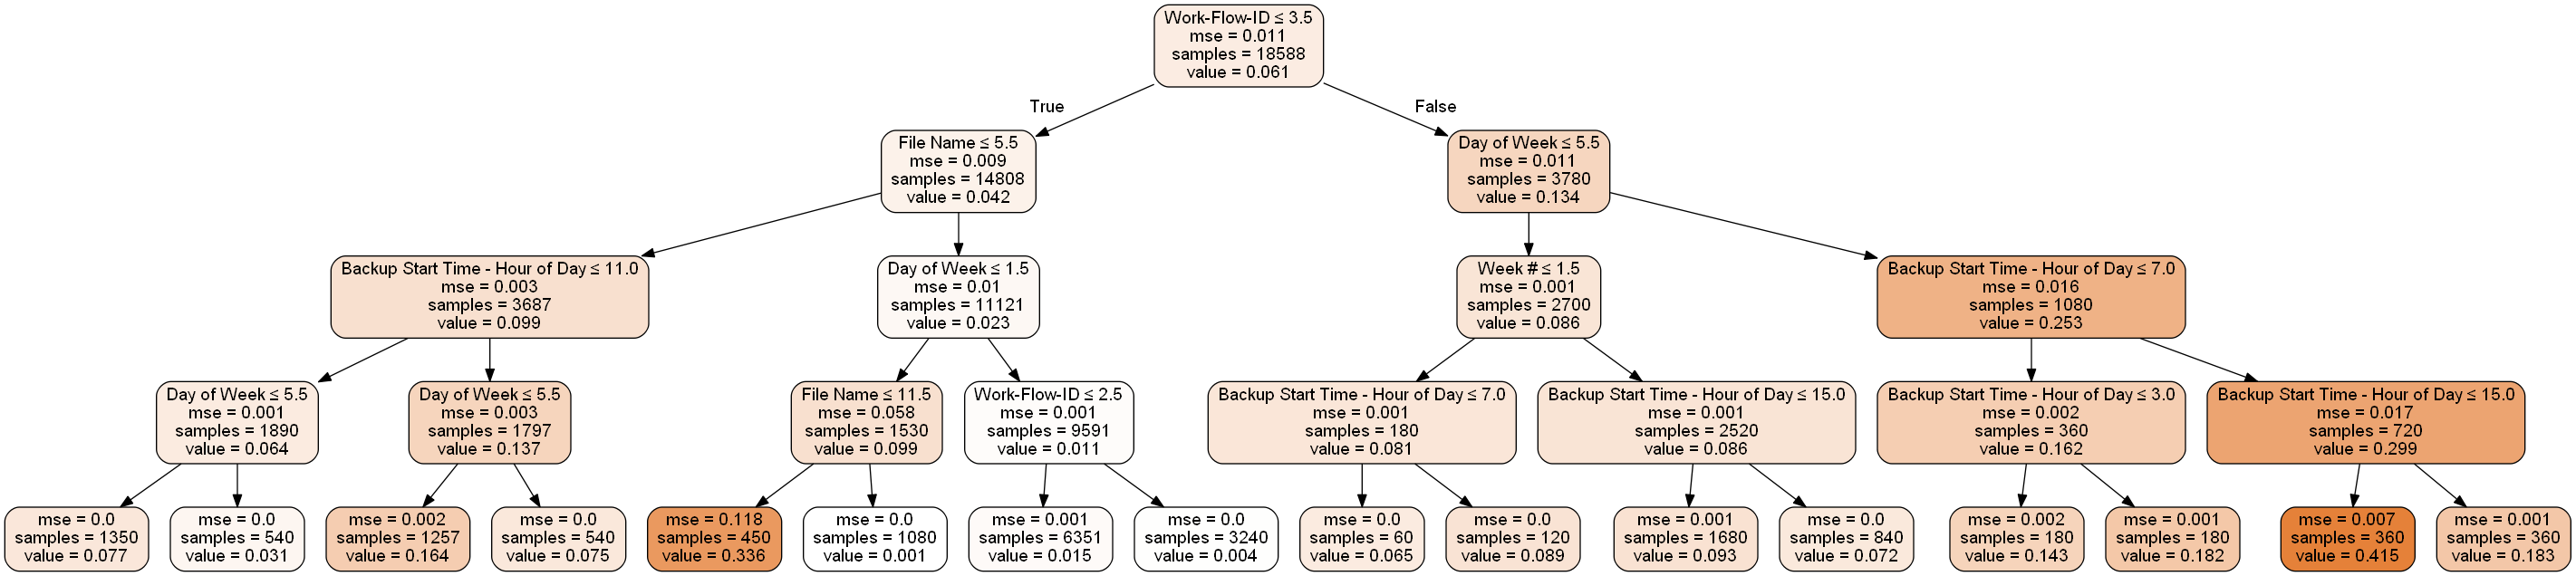
\includegraphics{Figure/2bv.png}}
\caption{Decision Tree} \label{2bv}
\end{figure}

\subsubsection{neural network regression model}

Now we used a neural network regression model with one hidden layer and all features one-hot encoded. Again we used k-folder cross-validation to find the optimal combination of the number of hiddens units and activation functions. We tried $2, 5, 10, 50, 100, 150, 200, 250, 300, 350, 400, 450, 500, 550, 600$ with relu, logistic, tanh. The plot of the test-RMSE against the number of hidden units for different activation functions is shown in Fig \ref{1_nn}.

The best model chosen from the cross-validation is a neural network model with $550$ hidden units and relu activation and the train and test RMSE are $0.04054727126423967$ and $0.03918910976276833$. The plot of fitted values against true values and residuals versus fitted values are shown in Fig \ref{1_nn1} and Fig \ref{1_nn2}.

\begin{figure}[!htbp]
\centering
\scalebox{0.4}{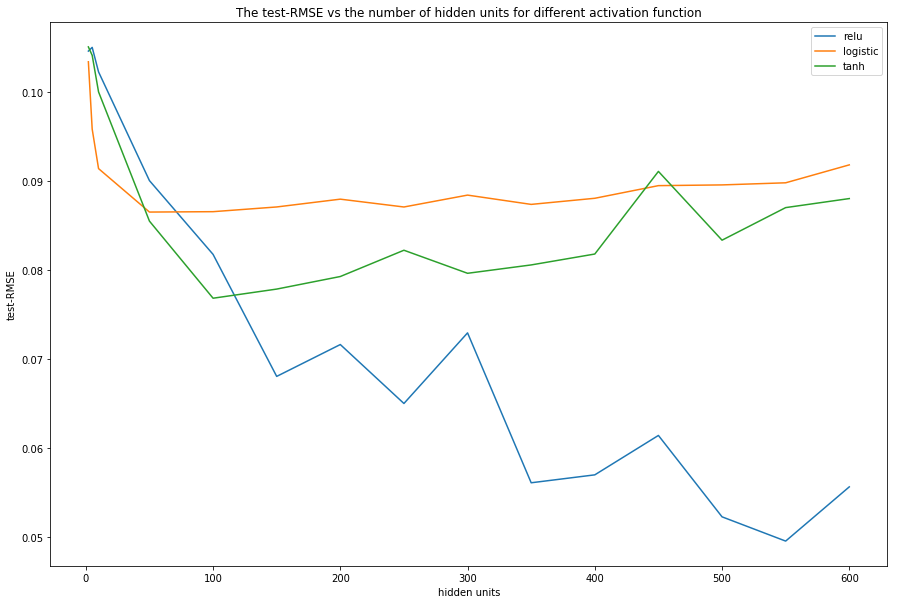
\includegraphics{Figure/1_nn.png}}
\caption{the test-RMSE against the number of hidden units for different activation functions} \label{1_nn}
\end{figure}

\begin{figure}[!htbp]
\centering
\scalebox{0.4}{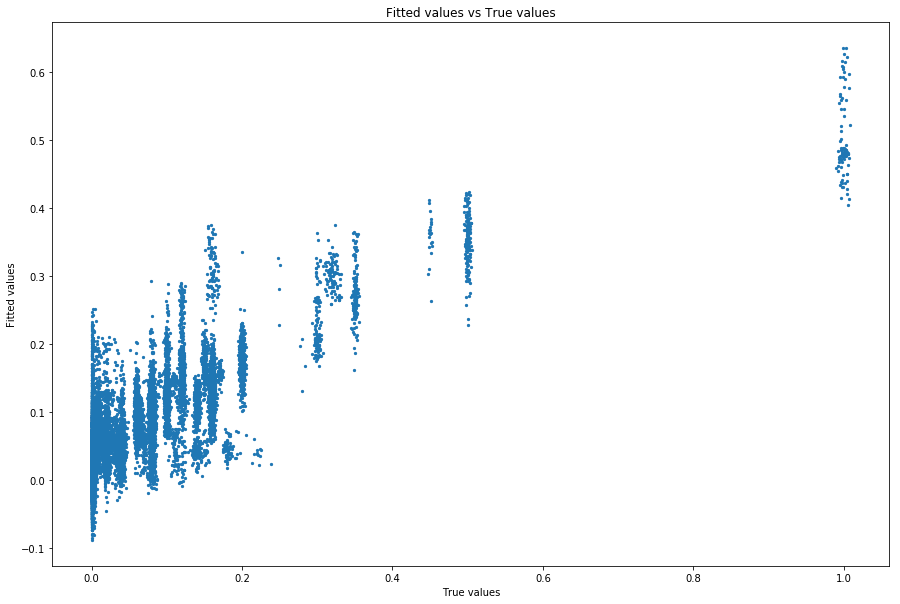
\includegraphics{Figure/1_nn1.png}}
\caption{fitted values against true values} \label{1_nn1}
\end{figure}

\begin{figure}[!htbp]
\centering
\scalebox{0.4}{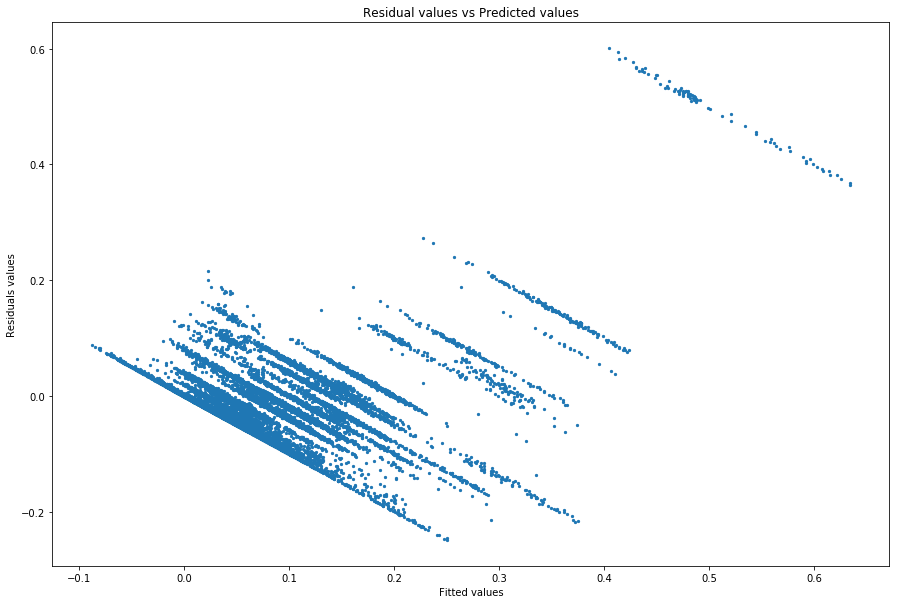
\includegraphics{Figure/1_nn2.png}}
\caption{residuals versus fitted values} \label{1_nn2}
\end{figure}

\subsubsection{separate workflows}

(i) This time we predicted the Backup size for each of the workflows separately. Using linear regression model, the scatter plot of those $5$ workflows are shown in Fig \ref{1d_01}, \ref{1d_02}, \ref{1d_11}, \ref{1d_12}, \ref{1d_21}, \ref{1d_22}, \ref{1d_31}, \ref{1d_32}, \ref{1d_41}, and \ref{1d_42}. The train and test error of each separate workflow can be seen in Table \ref{tab1}. We could see that the performance of the linear prediction model has been dramatically improved. This is very intuitive since each workflow may has each different inside parameters or models. By separating those difference the linear model would fit the data more accurately. 

\begin{table}[h]
\center
\caption{Train and test RMSE}
\scalebox{0.9}{
\begin{tabular}{c|c|c}
\hline
Workflow ID & train RMSE & test RMSE \\\hline
$0$ & $0.035836058473410995$ & $0.035864233365527486$ \\
$1$ & $0.14873667005167984$ & $0.14718022940875605$ \\
$2$ & $0.042912741990063744$ & $0.042871138232155256$ \\
$3$ & $0.007244122686732686$ & $0.007236474722628693$ \\
$4$ & $0.08591840773195633$ & $0.08587749300354083$
\end{tabular}}
\label{tab1}
\end{table}

\begin{figure}[!htbp]
\centering
\scalebox{0.4}{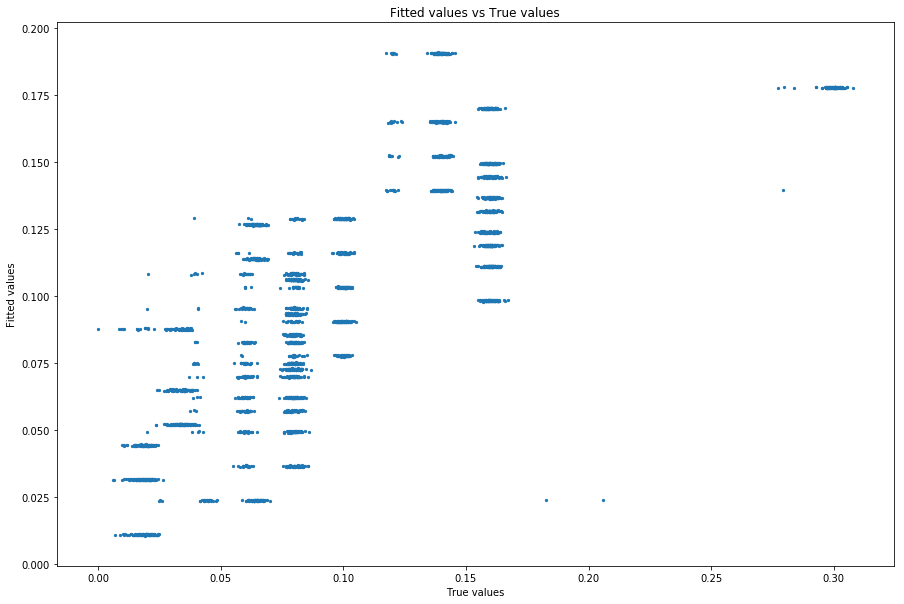
\includegraphics{Figure/1d_01.png}}
\caption{fitted values against true values for workflow $0$} \label{1d_01}
\end{figure}

\begin{figure}[!htbp]
\centering
\scalebox{0.4}{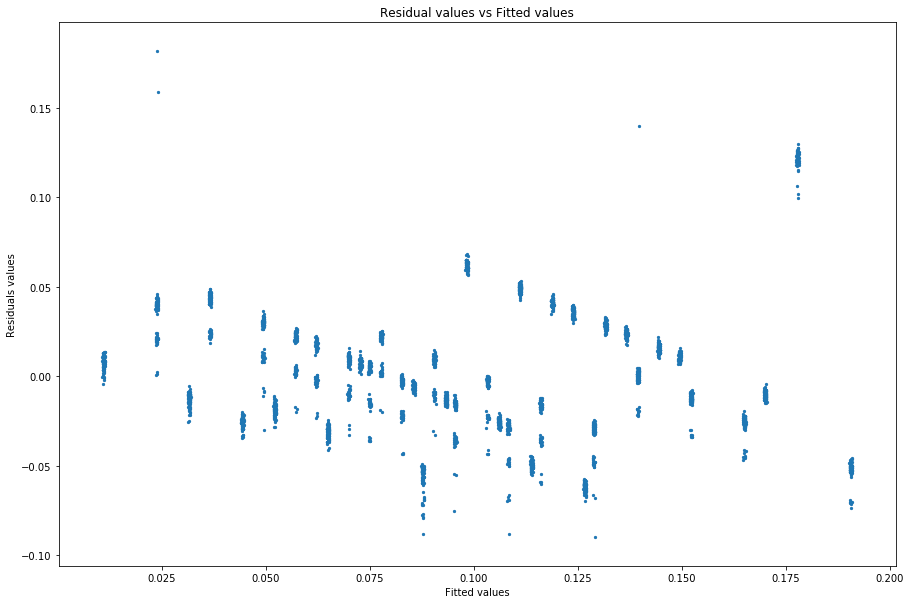
\includegraphics{Figure/1d_02.png}}
\caption{residuals versus fitted values for workflow $0$} \label{1d_02}
\end{figure}

\begin{figure}[!htbp]
\centering
\scalebox{0.4}{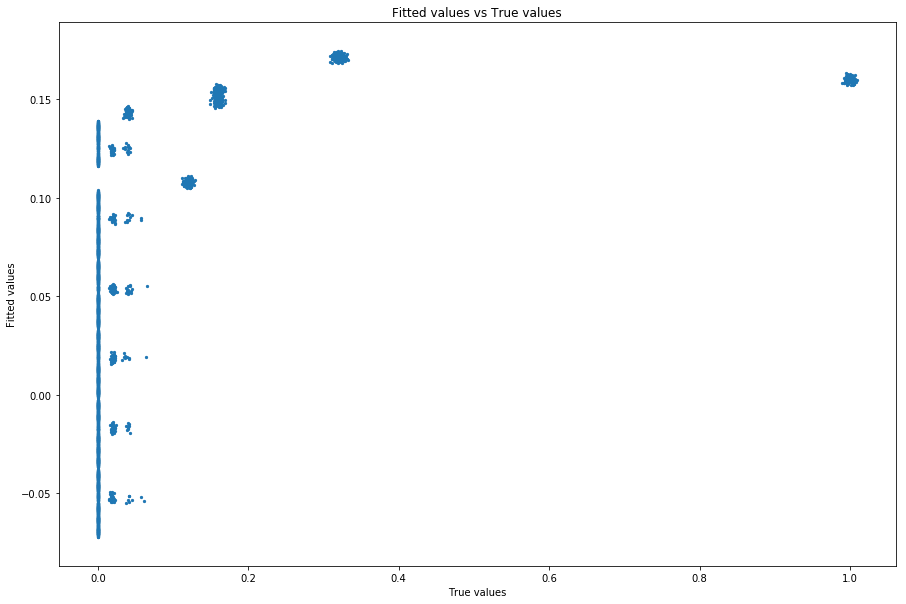
\includegraphics{Figure/1d_11.png}}
\caption{fitted values against true values for workflow $1$} \label{1d_11}
\end{figure}

\begin{figure}[!htbp]
\centering
\scalebox{0.4}{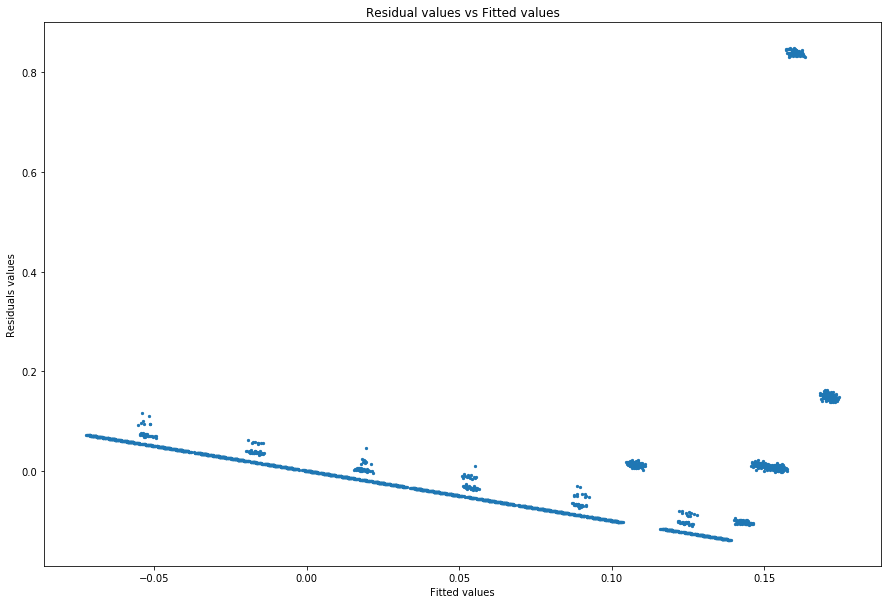
\includegraphics{Figure/1d_12.png}}
\caption{residuals versus fitted values for workflow $1$} \label{1d_12}
\end{figure}

\begin{figure}[!htbp]
\centering
\scalebox{0.4}{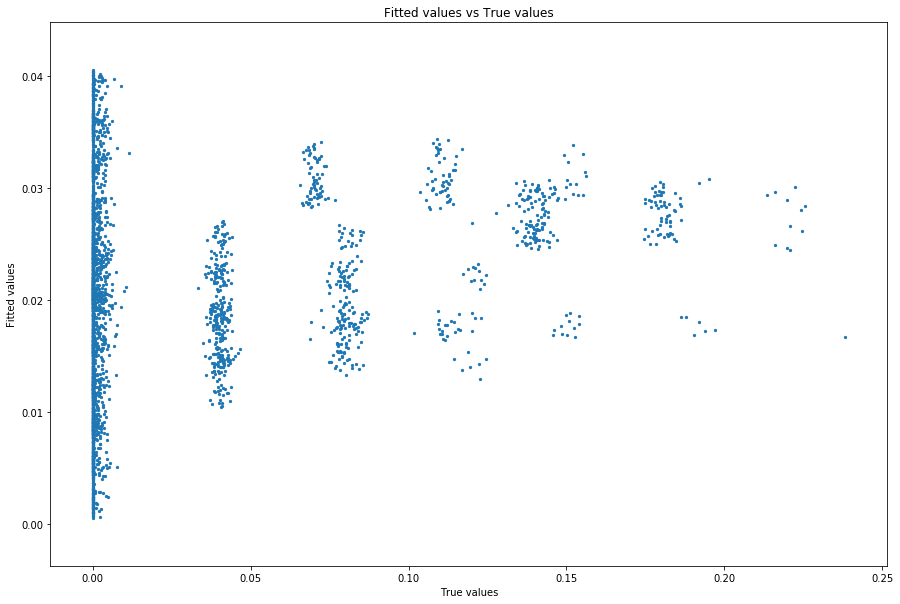
\includegraphics{Figure/1d_21.png}}
\caption{fitted values against true values for workflow $2$} \label{1d_21}
\end{figure}

\begin{figure}[!htbp]
\centering
\scalebox{0.4}{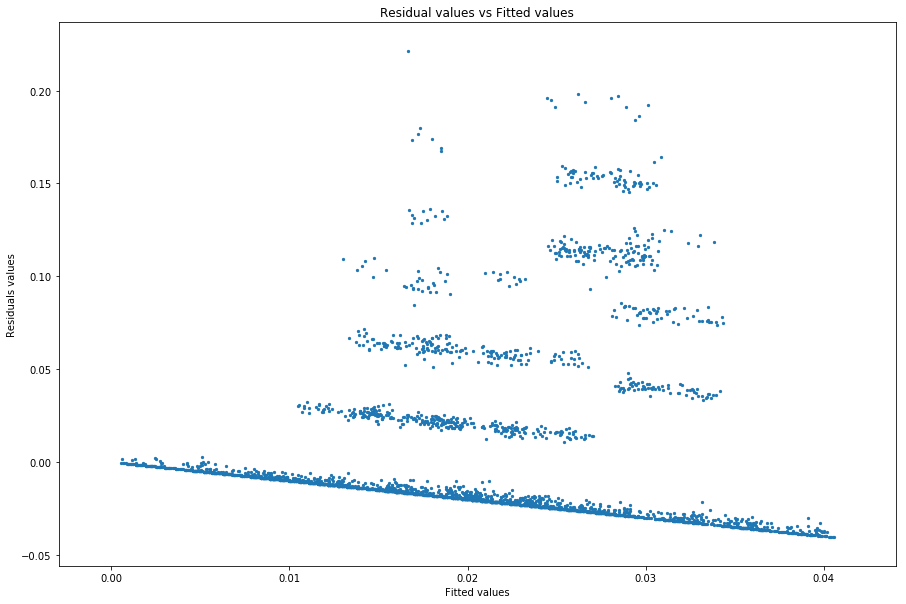
\includegraphics{Figure/1d_22.png}}
\caption{residuals versus fitted values for workflow $2$} \label{1d_22}
\end{figure}

\begin{figure}[!htbp]
\centering
\scalebox{0.4}{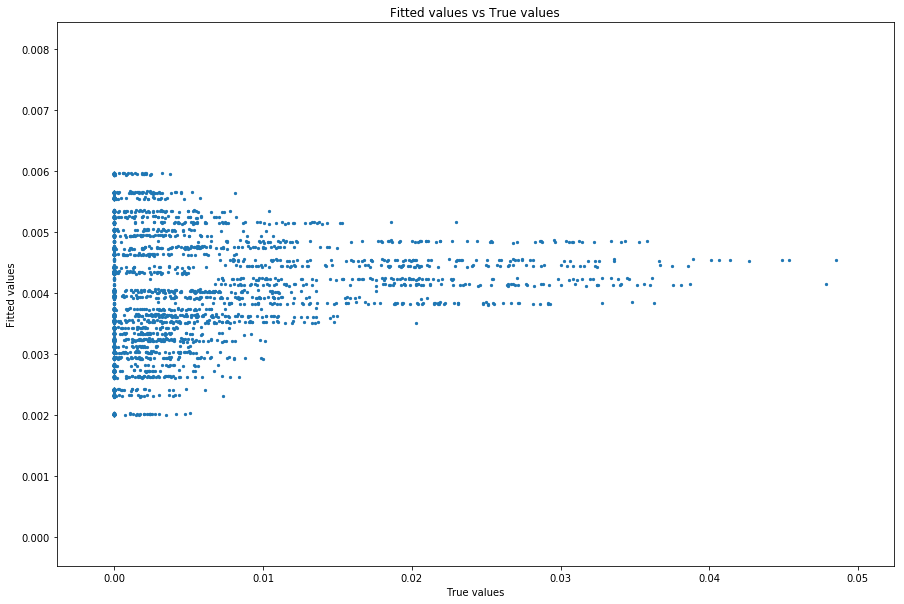
\includegraphics{Figure/1d_31.png}}
\caption{fitted values against true values for workflow $3$} \label{1d_31}
\end{figure}

\begin{figure}[!htbp]
\centering
\scalebox{0.4}{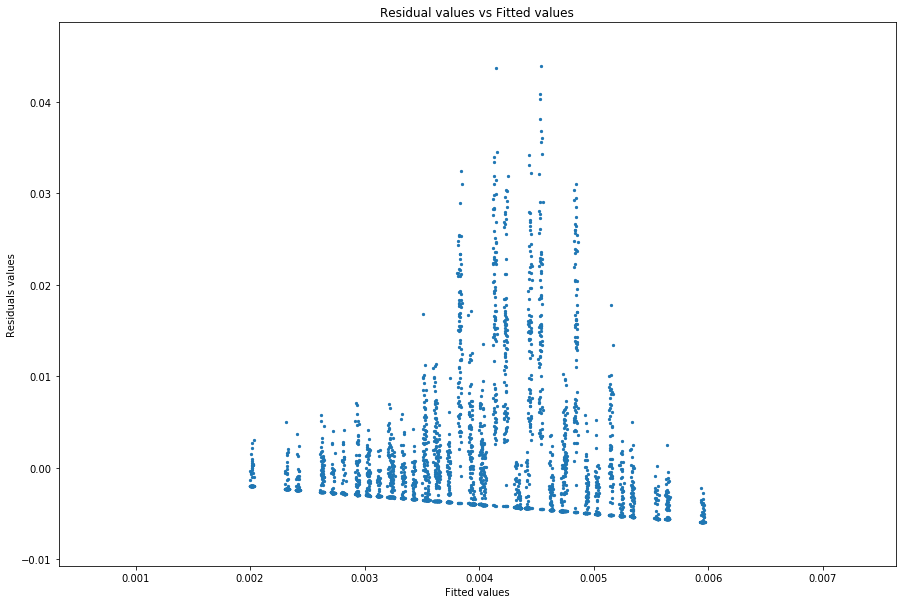
\includegraphics{Figure/1d_32.png}}
\caption{residuals versus fitted values for workflow $3$} \label{1d_32}
\end{figure}

\begin{figure}[!htbp]
\centering
\scalebox{0.4}{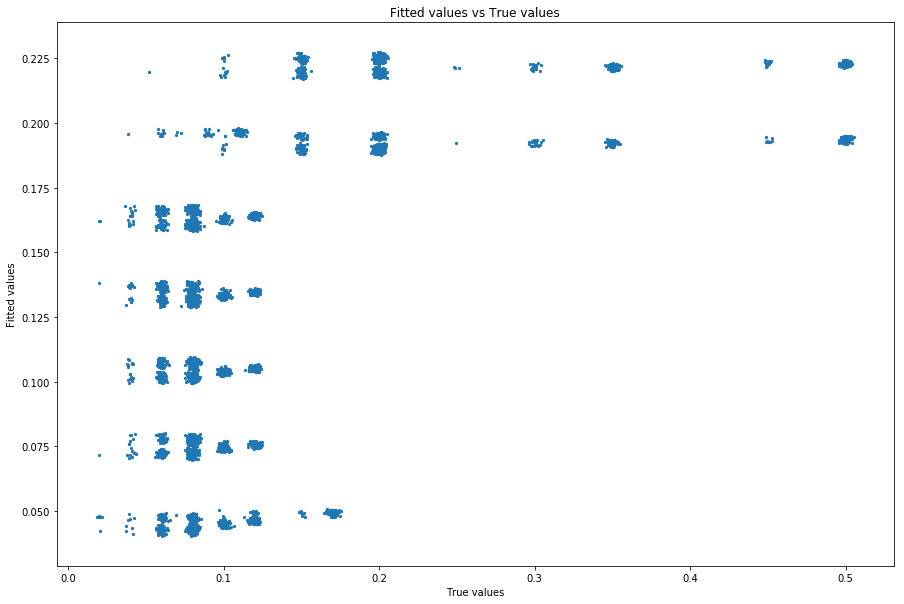
\includegraphics{Figure/1d_41.png}}
\caption{fitted values against true values for workflow $4$} \label{1d_41}
\end{figure}

\begin{figure}[!htbp]
\centering
\scalebox{0.4}{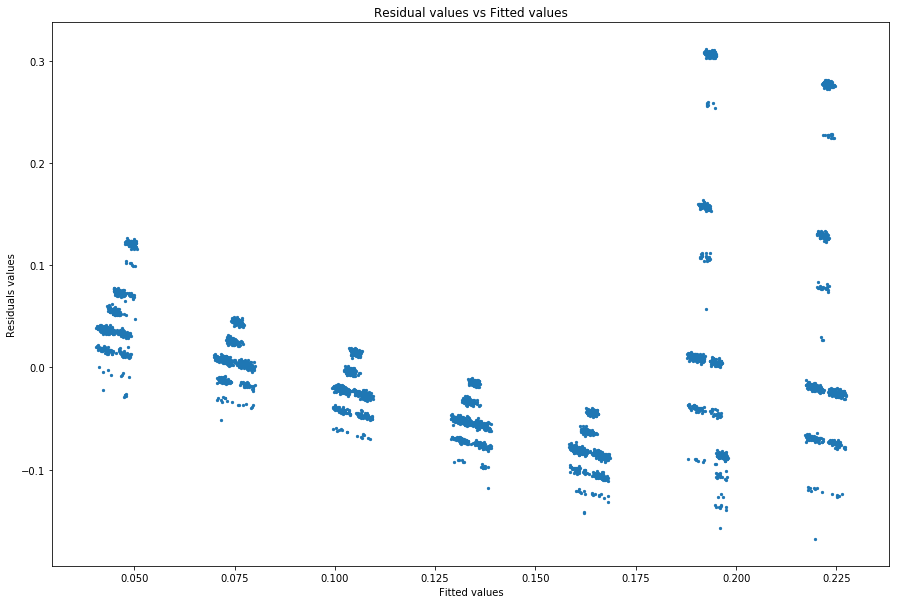
\includegraphics{Figure/1d_42.png}}
\caption{residuals versus fitted values for workflow $4$} \label{1d_42}
\end{figure}

(ii) We tried different degree of the polynomial of the model. The plot of the train and test RMSE against the degree is shown in Fig \ref{1d2_00}, \ref{1d2_10}, \ref{1d2_20}, \ref{1d2_30}, and \ref{1d2_40} separately. The train and test error and best degree that we find of each separate workflow can be seen in Table \ref{tab2}. It's obvious that as we increase the degree the training error can always decrease, which seems like a good thing but what comes aside is the overfitting problem. The plot proves it that the test error becomes increase if the degree is way too high.

\begin{table}[h]
\center
\caption{Train and test RMSE and best degree}
\scalebox{0.9}{
\begin{tabular}{c|c|c|c}
\hline
Workflow ID & degree & train RMSE & test RMSE \\\hline
$0$ & $8$ & $0.009215949356264234$ & $0.007952311037775975$ \\
$1$ & $9$ & $0.006489646031637972$ & $0.005441175333664292$ \\
$2$ & $9$ & $0.021160106836710026$ & $0.017828380830571006$ \\
$3$ & $7$ & $0.004682304240652268$ & $0.004377076086892894$ \\
$4$ & $9$ & $0.020306227755373964$ & $0.016098651643866833$ \\
\end{tabular}}
\label{tab2}
\end{table}


\begin{figure}[!htbp]
\centering
\scalebox{0.4}{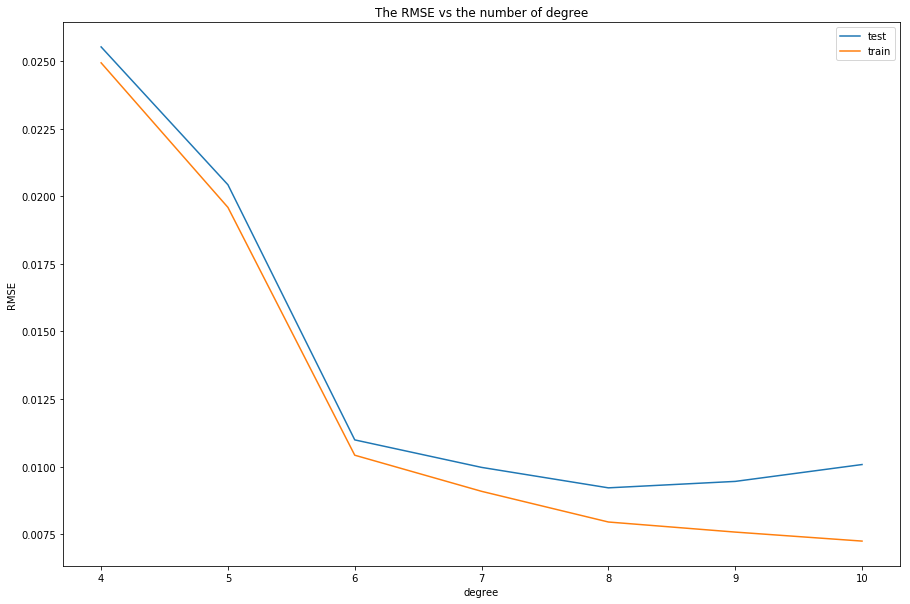
\includegraphics{Figure/1b2_00.png}}
\caption{the RMSE against the degree for workflow $0$} \label{1d2_00}
\end{figure}

\begin{figure}[!htbp]
\centering
\scalebox{0.4}{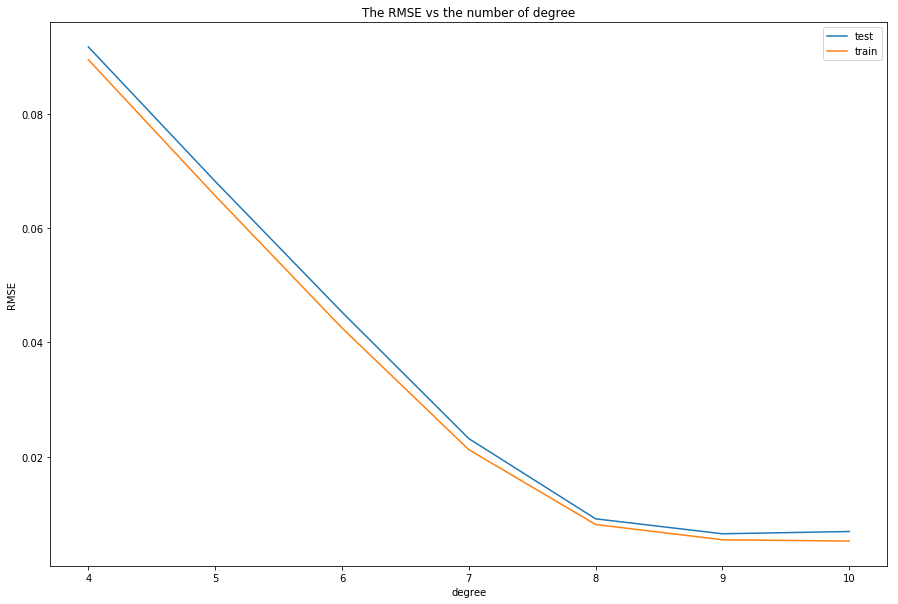
\includegraphics{Figure/1b2_10.png}}
\caption{the RMSE against the degree for workflow $1$} \label{1d2_10}
\end{figure}

\begin{figure}[!htbp]
\centering
\scalebox{0.4}{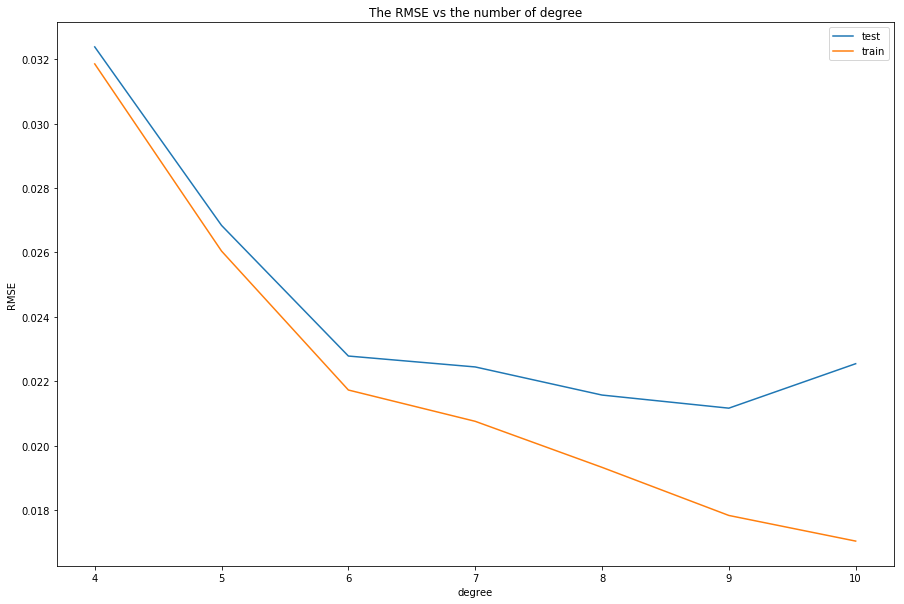
\includegraphics{Figure/1b2_20.png}}
\caption{the RMSE against the degree for workflow $2$} \label{1d2_20}
\end{figure}

\begin{figure}[!htbp]
\centering
\scalebox{0.4}{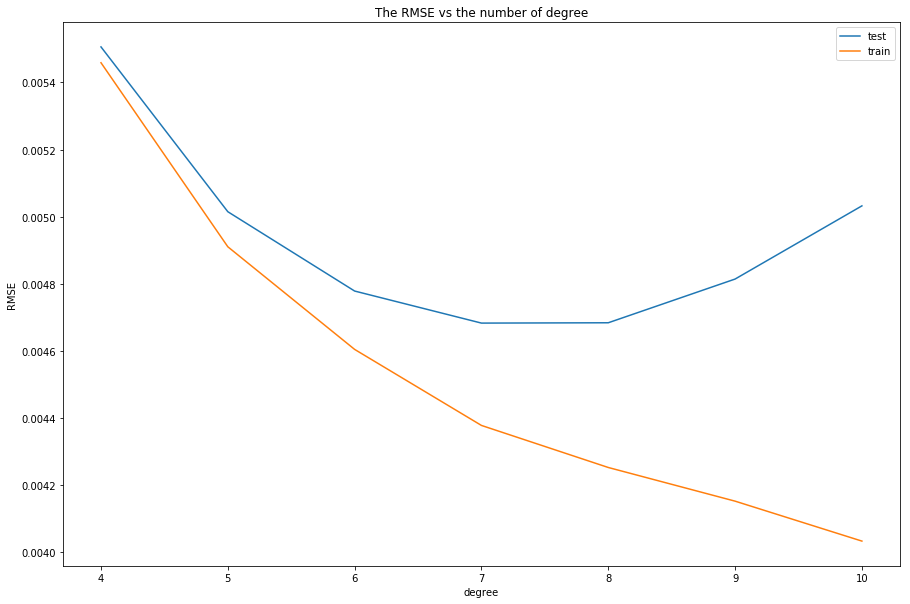
\includegraphics{Figure/1b2_30.png}}
\caption{the RMSE against the degree for workflow $3$} \label{1d2_30}
\end{figure}

\begin{figure}[!htbp]
\centering
\scalebox{0.4}{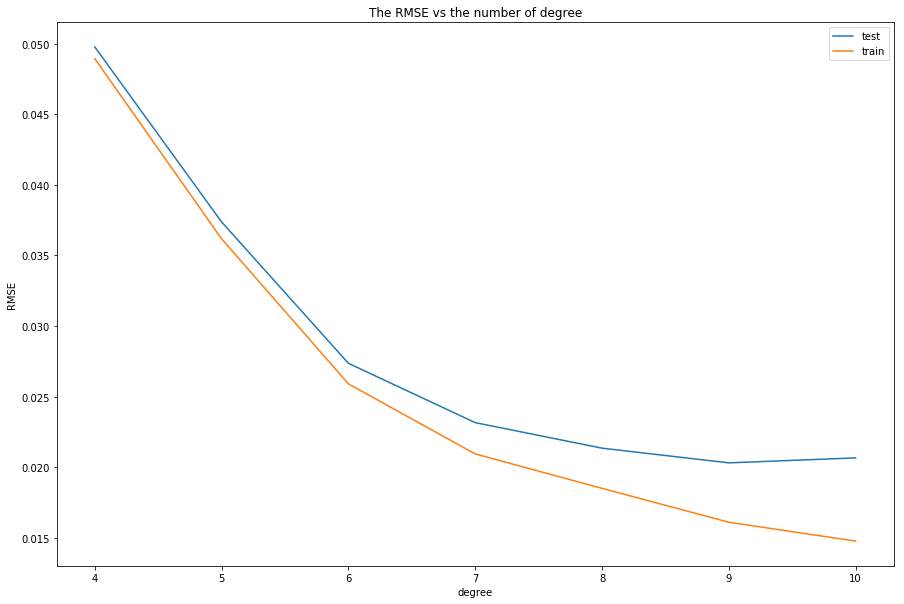
\includegraphics{Figure/1b2_40.png}}
\caption{the RMSE against the degree for workflow $4$} \label{1d2_40}
\end{figure}



The new scatter plot with best parameter for those $5$ workflows are shown in Fig \ref{1d2_01}, \ref{1d2_02}, \ref{1d2_11}, \ref{1d2_12}, \ref{1d2_21}, \ref{1d2_22}, \ref{1d2_31}, \ref{1d2_32}, \ref{1d2_41}, and \ref{1d2_42}.

\begin{figure}[!htbp]
\centering
\scalebox{0.4}{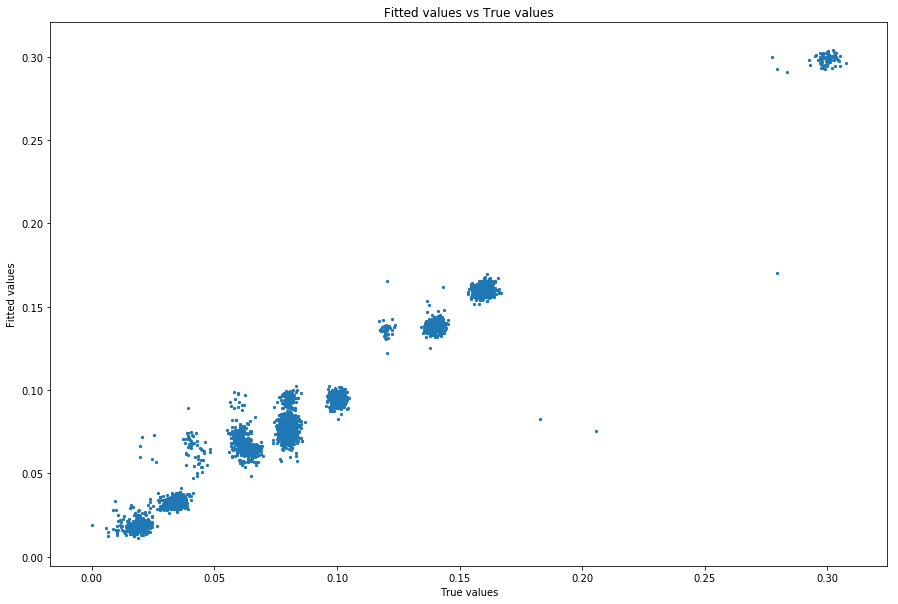
\includegraphics{Figure/1b2_01.png}}
\caption{fitted values against true values for workflow $0$} \label{1d2_01}
\end{figure}

\begin{figure}[!htbp]
\centering
\scalebox{0.4}{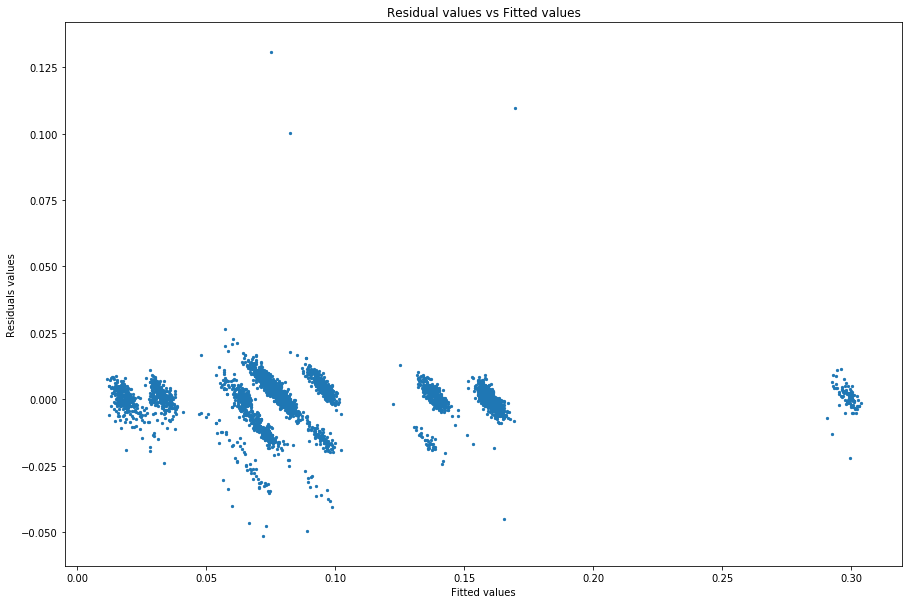
\includegraphics{Figure/1b2_02.png}}
\caption{residuals versus fitted values for workflow $0$} \label{1d2_02}
\end{figure}

\begin{figure}[!htbp]
\centering
\scalebox{0.4}{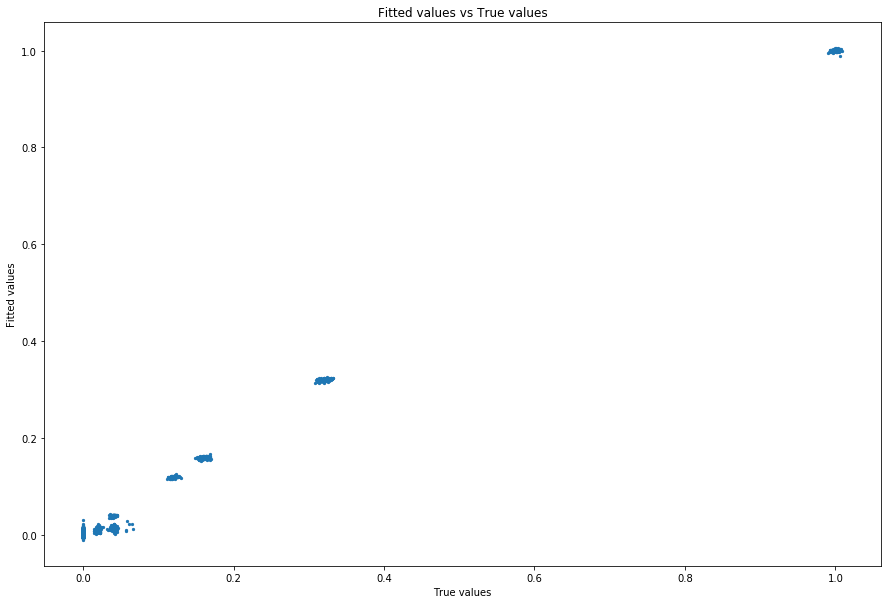
\includegraphics{Figure/1b2_11.png}}
\caption{fitted values against true values for workflow $1$} \label{1d2_11}
\end{figure}

\begin{figure}[!htbp]
\centering
\scalebox{0.4}{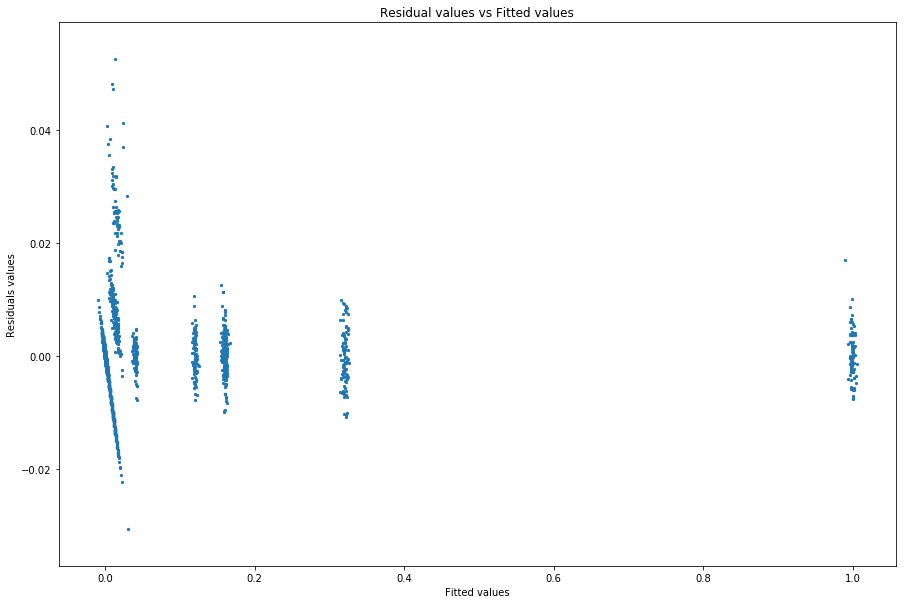
\includegraphics{Figure/1b2_12.png}}
\caption{residuals versus fitted values for workflow $1$} \label{1d2_12}
\end{figure}

\begin{figure}[!htbp]
\centering
\scalebox{0.4}{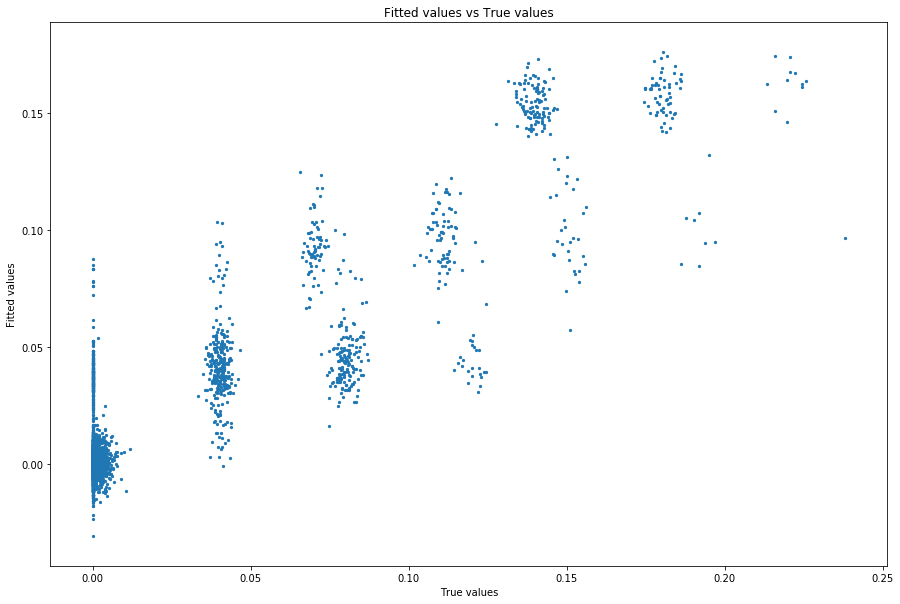
\includegraphics{Figure/1b2_21.png}}
\caption{fitted values against true values for workflow $2$} \label{1d2_21}
\end{figure}

\begin{figure}[!htbp]
\centering
\scalebox{0.4}{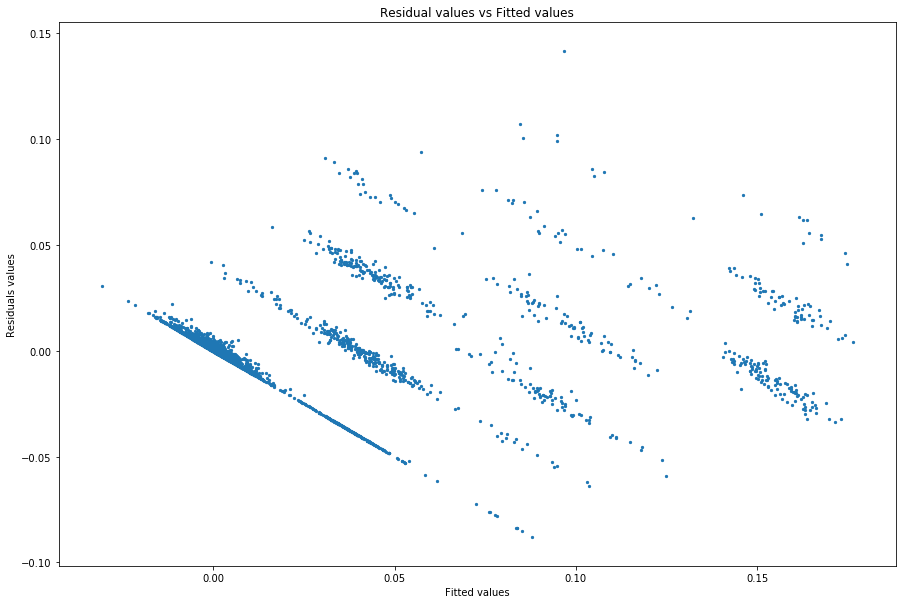
\includegraphics{Figure/1b2_22.png}}
\caption{residuals versus fitted values for workflow $2$} \label{1d2_22}
\end{figure}

\begin{figure}[!htbp]
\centering
\scalebox{0.4}{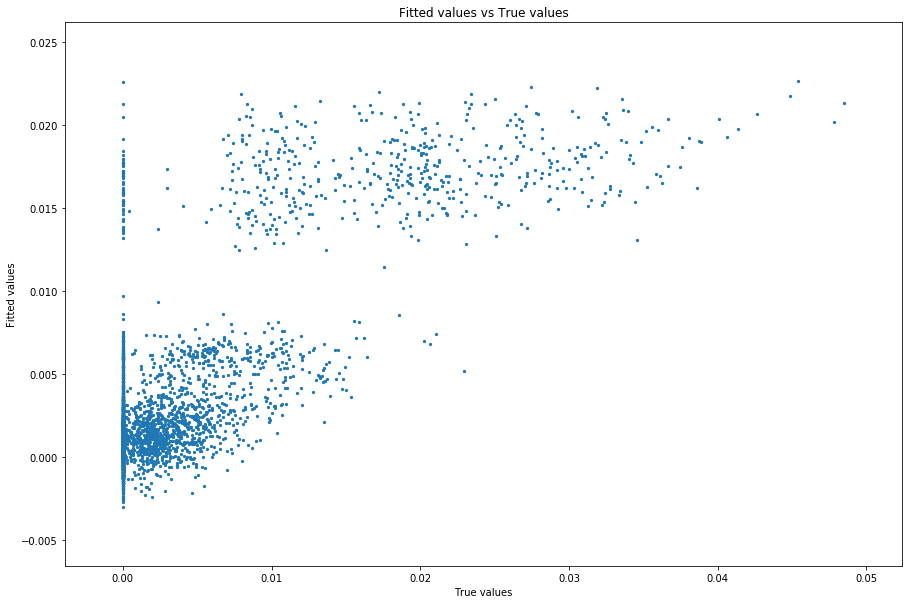
\includegraphics{Figure/1b2_31.png}}
\caption{fitted values against true values for workflow $3$} \label{1d2_31}
\end{figure}

\begin{figure}[!htbp]
\centering
\scalebox{0.4}{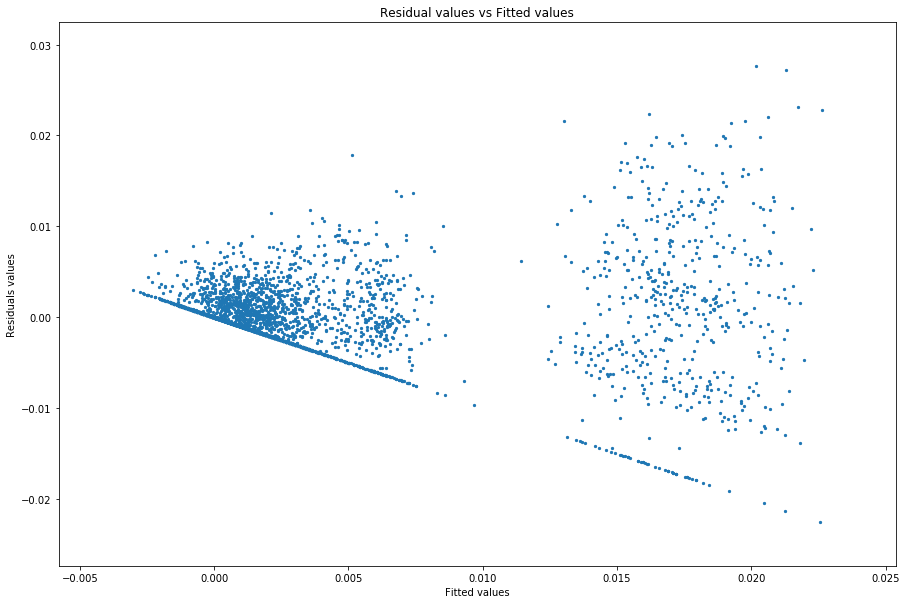
\includegraphics{Figure/1b2_32.png}}
\caption{residuals versus fitted values for workflow $3$} \label{1d2_32}
\end{figure}

\begin{figure}[!htbp]
\centering
\scalebox{0.4}{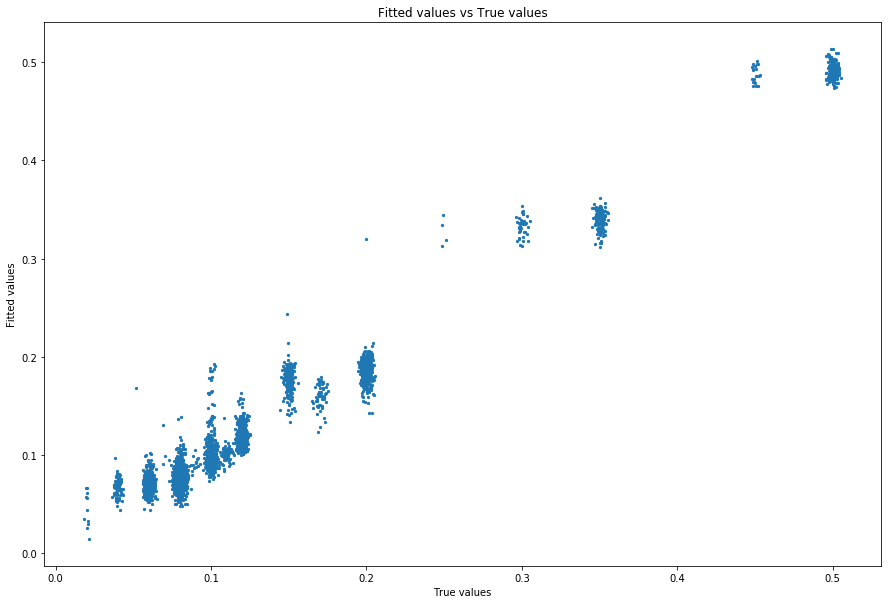
\includegraphics{Figure/1b2_41.png}}
\caption{fitted values against true values for workflow $4$} \label{1d2_41}
\end{figure}

\begin{figure}[!htbp]
\centering
\scalebox{0.4}{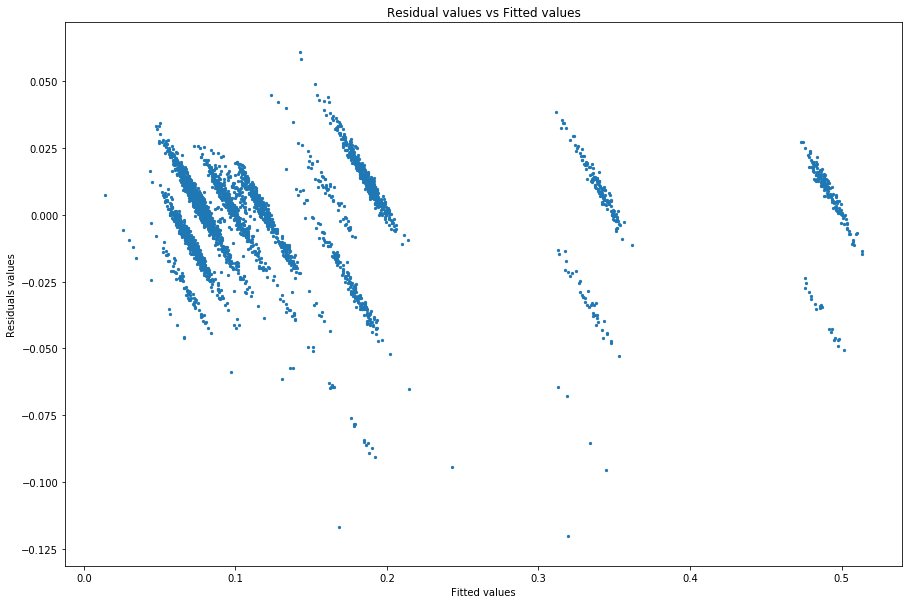
\includegraphics{Figure/1b2_42.png}}
\caption{residuals versus fitted values for workflow $4$} \label{1d2_42}
\end{figure}


\subsubsection{k-nearest neighbor regression}

Using k-nearest neighbor regression, the plot of the test-RMSE against the number of neighbor is shown in Fig \ref{1_kn}. The best parameter is $4$ and the train and test RMSE of that model are $0.03509321892803684$ and $0.027896132153362275$. The plot of fitted values against true values and residuals versus fitted values are shown in Fig \ref{1_kn1} and Fig \ref{1_kn2}.


\begin{figure}[!htbp]
\centering
\scalebox{0.4}{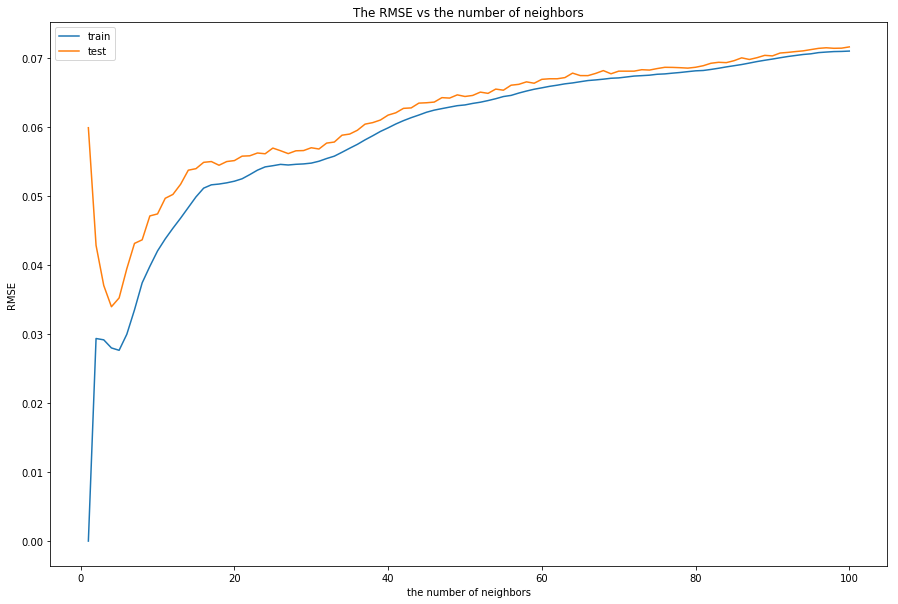
\includegraphics{Figure/1_kn.png}}
\caption{the test-RMSE against the number of neighbor} \label{1_kn}
\end{figure}

\begin{figure}[!htbp]
\centering
\scalebox{0.4}{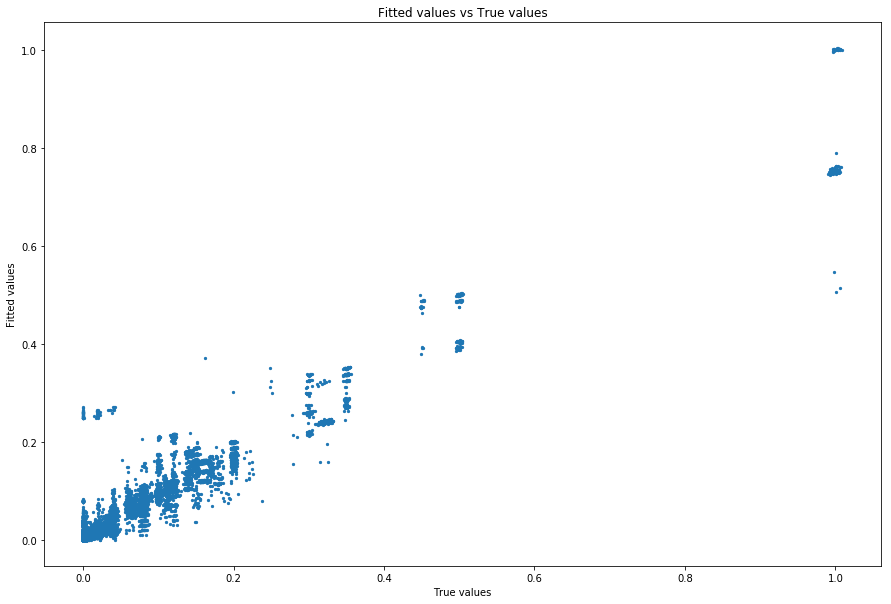
\includegraphics{Figure/1_kn1.png}}
\caption{fitted values against true values} \label{1_kn1}
\end{figure}

\begin{figure}[!htbp]
\centering
\scalebox{0.4}{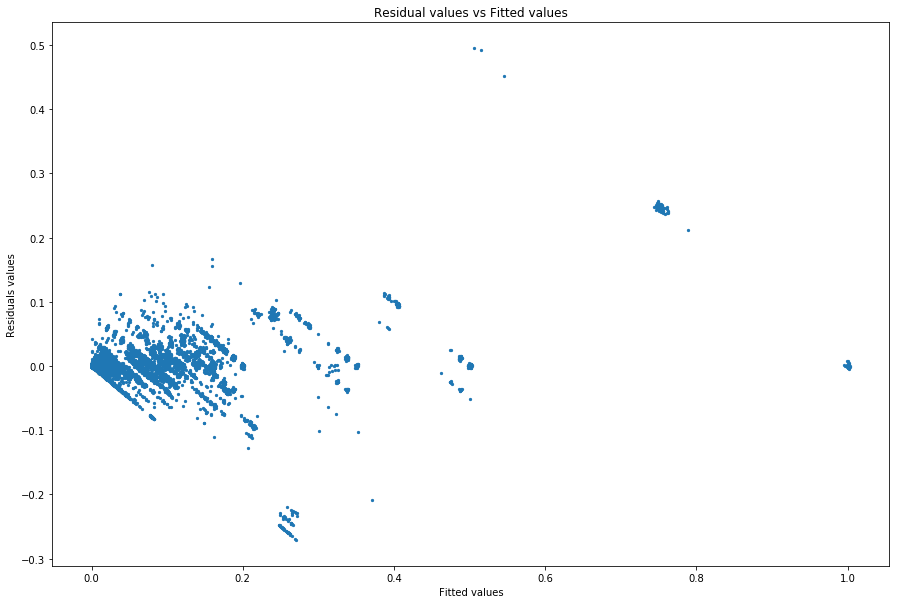
\includegraphics{Figure/1_kn2.png}}
\caption{residuals versus fitted values} \label{1_kn2}
\end{figure}

\subsection{Compare these regression models}

The performance of all these regression models we discussed before can be found in Table \ref{tab3}. We could conclude from the observation that the random forest, neural network and knn all give us good enough performance under the measurement of test RMSE. Even though the original linear model doesn't work well, we still can extremely improve it by separating each workflow and increasing the degrees of the model.

\begin{table}[h]
\center
\caption{Best train and test RMSE among all regression models}
\scalebox{0.9}{
\begin{tabular}{c|c|c}
\hline
model & train RMSE & test RMSE \\\hline
linear & $0.10358719585332854$ & $0.10358269769007267$ \\\hline
linear workflow $0$ & $0.035836058473410995$ & $0.035864233365527486$ \\
linear workflow $1$ & $0.14873667005167984$ & $0.14718022940875605$ \\
linear workflow $2$ & $0.042912741990063744$ & $0.042871138232155256$ \\
linear workflow $3$ & $0.007244122686732686$ & $0.007236474722628693$ \\
linear workflow $4$ & $0.08591840773195633$ & $0.08587749300354083$\\\hline
high degree linear workflow $0$ & $0.009215949356264234$ & $0.007952311037775975$ \\
high degree linear workflow $1$ & $0.006489646031637972$ & $0.005441175333664292$ \\
high degree linear workflow $2$ & $0.021160106836710026$ & $0.017828380830571006$ \\
high degree linear workflow $3$ & $0.004682304240652268$ & $0.004377076086892894$ \\
high degree linear workflow $4$ & $0.020306227755373964$ & $0.016098651643866833$ \\\hline
random forest & $0.021061323772690425$ & $0.021657162672114462$ \\\hline
neural network & $0.04054727126423967$ & $0.03918910976276833$ \\\hline
k-nearest neighbour & $0.03509321892803684$ & $0.027896132153362275$. \\
\end{tabular}}
\label{tab3}
\end{table}


\newpage

\section{Boston Housing Dataset}
\subsection{Load the dataset}
\subsection{Fit a linear regression model}

\bigbreak 
The F-values and p-values are:\\

F = [ 89.27867007  75.08340878 153.982021    15.95925779 112.35134671 470.92252602  83.29994976 33.50345866  85.77751739 141.48567511 175.33780624  62.90074607 602.30110356]\\

p = [1.29165892e-19 6.19893794e-17 4.93018661e-31 7.43915002e-05 7.87623345e-24 3.45360629e-74 1.70543500e-18 1.25304781e-08 5.83365934e-19 6.37376693e-29 1.50648864e-34 1.41751808e-14 4.90947265e-88]\\

The variable that has a low p-value is likely to be significant. Conversely, a larger p-value suggests the variable is likely to be insignificant. So the order of significance of variables is: $LSTAT>RM>PTRATIO>INDUS>TAX>NOX>CRIM>RAD>AGE>ZN>B>DIS>CHAS$\\

Averaged Root Mean Squared Errors of test and training are: 
Average test RMSE: 5.191327655559577 ; Average training RMSE: 4.605185401794117

\begin{figure}[!htbp]
\centering
\scalebox{0.7}{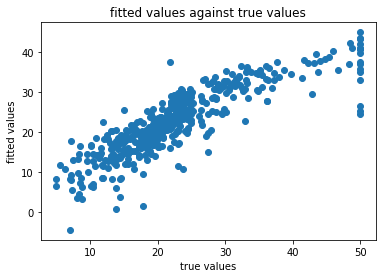
\includegraphics{Figure/d2_f1.png}}
\caption{fitted values against true values} \label{dataset2_1}
\end{figure}

\begin{figure}[!htbp]
\centering
\scalebox{0.7}{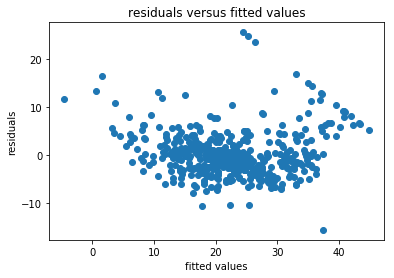
\includegraphics{Figure/d2_f2.png}}
\caption{residuals versus fitted values} \label{dataset2_2}
\end{figure}

Scatter plots of fitted values against true values and residuals versus fitted values using the whole dataset can be seen in figure \ref{dataset2_1} and figure \ref{dataset2_2}.
\newline


\subsection{Control overfitting via regularization of the parameters}
\bigbreak 
After trying different values, best choices of $\alpha$, $\lambda1$, $\lambda2$ and corresponding RMSEs obtained via 10-fold cross validation and estimated coefficients are:\\\\
Regularization method: Ridge\\
Best parameter Test RMSE:  5.037718653318939\\
Best parameter Train RMSE:  4.842570572044513\\
Best $\alpha$:  100\\
Estimated coefficients:  [-9.87348682e-02  5.75000733e-02 -5.24367753e-02  6.30453235e-01 -2.50839386e-01  2.20491982e+00 -1.13944138e-04 -1.23509929e+00 3.09145266e-01 -1.55229229e-02 -8.01378743e-01  9.38365517e-03 -6.94791951e-01]\\\\
Regularization method: Lasso\\
Best parameter Test RMSE:  5.1083599482410325\\
Best parameter Train RMSE:  4.729257067596344\\
Best $\alpha$:  0.1\\
Estimated coefficients:  [-0.09499876  0.05404697 -0.03796886  1.1136662  -0.          3.55262497 -0.01277121 -1.2804953   0.2682344  -0.01408458 -0.7423286   0.01017644 -0.60427997]\\\\
Regularization method: Elastic Net\\
Best parameter Test RMSE:  5.022347107449401\\
Best parameter Train RMSE:  4.761934847801649\\
Best $\alpha$:  0.1\\
Best l1Ratio:  0\\
Best $\lambda1$:  0.0\\
Best $\lambda2$:  0.05\\
Estimated coefficients:  [-0.0989382   0.05676159 -0.04914643  1.05795062 -0.55761236  2.85560729 -0.00776635 -1.30952237  0.29329637 -0.01473338 -0.7874883   0.0097517 -0.64968596]\\

Estimated coefficients of unregularized best model are:  [-1.06498784e-01  5.14808179e-02 2.90518248e-02  2.69067244e+00 -1.80855060e+01  3.66226749e+00 -1.00886887e-03 -1.57259804e+00 3.09021741e-01 -1.19639182e-02 -9.72294752e-01  9.43731639e-03 -5.54185329e-01]\\

Among the three kinds regularization, the one that has smallest test RMSE is Elastic Net Regularizer with parameter $\lambda1$=0.0, $\lambda2$=0.05. And the best RMSE is 5.02235.
(Annotation: Here I justify why best $\alpha$ for Ridge is 100 whereas best $\lambda2$ for Elastic Net is 0.05. I found the test RMSE varies little when $\alpha$ changes from 0.1 to 100 for Ridge. The test RMSEs for $\alpha$=0.1,1,10,100 are 5.170394749496701, 5.0966971203549285, 5.054582577537348, 5.037718653318939,respectively.)\\

On the whole, the values of the estimated coefficients for these regularized good models are smaller than those of unregularized best model.(Most coefficients of the former are smaller than the latter, although some are not.) The reason is that we add the norm of coefficients to the cost function.



\newpage

\section{Car Insurance Dataset}
\subsection{Feature Preprocessing}

\noindent \textbf{(a) Feature Encoding} \bigbreak

\begin{figure}[!htbp]
\centering
\scalebox{0.4}{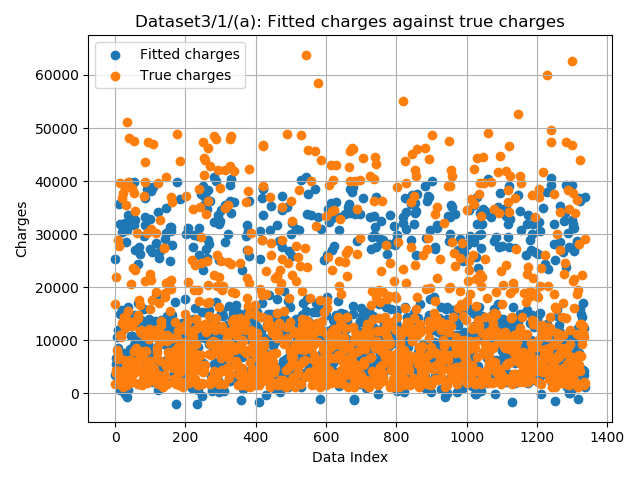
\includegraphics{Figure/3_1_a_1.png}}
\caption{Fitted charges against true charges without standardizing categorical features} \label{3_1_a_1}
\end{figure}

\begin{figure}[!htbp]
\centering
\scalebox{0.4}{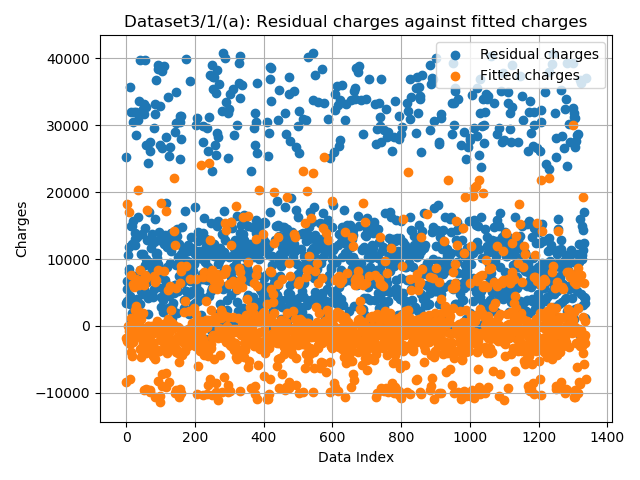
\includegraphics{Figure/3_1_a_2.png}}
\caption{Residual charges against fitted charges without standardizing categorical features} \label{3_1_a_2}
\end{figure}

Average training RMSE: 6045.093.\newline
\indent Average testing RMSE: 6082.919.\newline
\indent The fitted against true charges plot and residual plot suggest that the linear regression does not fit  very well.\bigbreak

\noindent \textbf{(b) Standardization} \bigbreak

\begin{figure}[!htbp]
\centering
\scalebox{0.4}{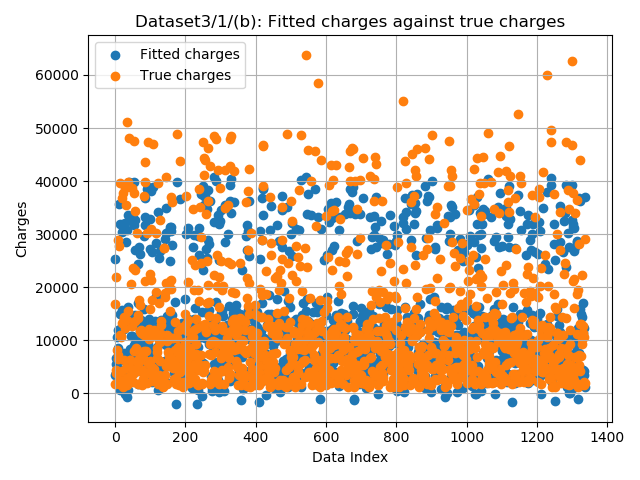
\includegraphics{Figure/3_1_b_1.png}}
\caption{Fitted charges against true charges with standardizing categorical features} \label{3_1_b_1}
\end{figure}

\begin{figure}[!htbp]
\centering
\scalebox{0.4}{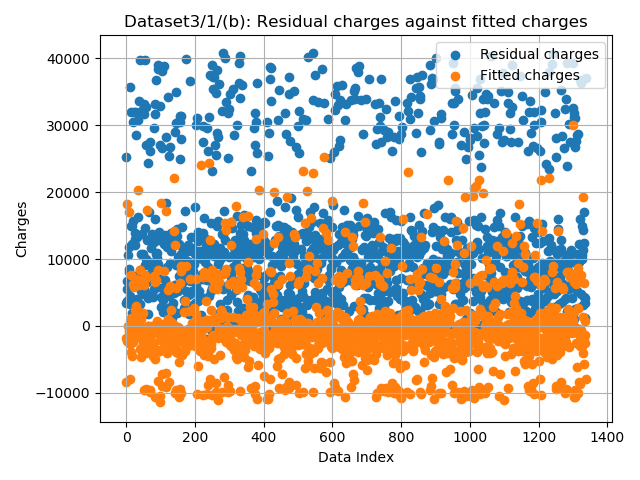
\includegraphics{Figure/3_1_b_2.png}}
\caption{Residual charges against fitted charges with standardizing categorical features} \label{3_1_b_2}
\end{figure}

Average training RMSE: 6045.093.\newline
\indent Average testing RMSE: 6082.919.\newline
\indent After standardization, the testing and training RMSE are still the same as before standardization. After we plot the fitted against true value and residual, the plots look the same as before standardization as well. With the standardization for linear regression, we get the exact same model, and thus same accuracy. This is why we get same testing RMSE, training RMSE, and same graphs.\bigbreak

\noindent \textbf{(c) Divide Numerical Features} \bigbreak

\begin{figure}[!htbp]
\centering
\scalebox{0.4}{\includegraphics{Figure/3_1_c_1.png}}
\caption{Fitted charges against true charges with dividing feature 1} \label{3_1_c_1}
\end{figure}

\begin{figure}[!htbp]
\centering
\scalebox{0.4}{\includegraphics{Figure/3_1_c_2.png}}
\caption{Residual charges against fitted charges with dividing feature 1} \label{3_1_c_2}
\end{figure}

Average training RMSE: 6198.081.\newline
\indent Average testing RMSE: 6240.027.\newline
\indent After dividing feature 1 into 3 levels, the training and testing RMSE got worse. The reason behind is probably due to a loss of information brought by such discretization.\bigbreak

\subsection{Correlation Exploration}

\noindent \textbf{(a)} \bigbreak

We use f regression and mutual information regression to select the two most important variables respectively. And we get:\newline
\indent F: 131.174, 54.709, 6.206, 4.400, 2177.615, 3.379\newline
\indent Mutual information: 1.500, 0.075, 0.161, 0.177, 0.369, 0.076\newline
\indent They all suggest that the first and fifth feafures are the most important ones selected.\bigbreak

\noindent \textbf{(b)} \bigbreak

\begin{figure}[!htbp]
\centering
\scalebox{0.4}{\includegraphics{Figure/3_2_b_1.png}}
\caption{Charges against features 2 and color points based on feature 5} \label{3_2_b_1}
\end{figure}

The figure can be found at \ref{3_2_b_1}. It seems that the feature 2 whose feature 5 value is 0 has a seemingly linear relation with charges.\bigbreak

\noindent \textbf{(c)} \bigbreak

\begin{figure}[!htbp]
\centering
\scalebox{0.4}{\includegraphics{Figure/3_2_c_1.png}}
\caption{Charges against features 1 and color points based on feature 5} \label{3_2_c_1}
\end{figure}

The figure can be found at \ref{3_2_c_1}. It seems that the feature 1 also has a seemingly linear relation with charges.\bigbreak

\subsection{Modify the Target Variable}

\noindent \textbf{(a)} \bigbreak

\begin{figure}[!htbp]
\centering
\scalebox{0.4}{\includegraphics{Figure/3_3_a_1.png}}
\caption{Fitted log of charges against true log of charges} \label{3_3_a_1}
\end{figure}

\begin{figure}[!htbp]
\centering
\scalebox{0.4}{\includegraphics{Figure/3_3_a_2.png}}
\caption{Residual log of charges against fitted log of charges} \label{3_3_a_2}
\end{figure}

Average training RMSE: 8359.526.\newline
\indent Average testing RMSE: 8437.228.\newline
\indent The preprocessing we picked is standardizing all these numerical features and keeping the one-hot-encoded features. It seems from the results above that this technique failed to bring any improvement to the regression performance.\bigbreak

\noindent \textbf{(b)} \bigbreak

We use f regression and mutual information regression to select the two most important variables respectively. And we get:\newline
\indent F: 515.977, 23.936, 35.705, 0.042, 1062.124, 2.923\newline
\indent Mutual information: 1.501, 0.067, 0.161, 0.176, 0.369, 0.078\newline
\indent They all once again suggest that the first and fifth feafures are the most important ones selected.\bigbreak

\subsection{Bonus Questions}

\noindent \textbf{(a)} \bigbreak

\begin{figure}[!htbp]
\centering
\scalebox{0.4}{\includegraphics{Figure/3_4_a_1.png}}
\caption{Fitted charges against true charges using polynomial features} \label{3_4_a_1}
\end{figure}

\begin{figure}[!htbp]
\centering
\scalebox{0.4}{\includegraphics{Figure/3_4_a_2.png}}
\caption{Residual charges against fitted charges using polynomial features} \label{3_4_a_2}
\end{figure}

Average training RMSE: 5999.819.\newline
\indent Average testing RMSE: 6052.478.\newline
\indent After trying polynomial features (applied on feature 1 and feature 5 with a factor of 2), the regression performance is successfully improved. These two features are selected based on the f regression and mutual information analysis conducted above. The possible reason for this improvement is probably due to the fact that the weights of the two most important features are increased, thus bringing more effective information to the regression model.\bigbreak

\noindent \textbf{(b) Random Forest} \bigbreak

\begin{figure}[!htbp]
\centering
\scalebox{0.4}{\includegraphics{Figure/3_4_b_RF_1.png}}
\caption{Fitted charges against true charges using random forest} \label{3_4_b_RF_1}
\end{figure}

\begin{figure}[!htbp]
\centering
\scalebox{0.4}{\includegraphics{Figure/3_4_b_RF_2.png}}
\caption{Residual charges against fitted charges using random forest} \label{3_4_b_RF_2}
\end{figure}

Average training RMSE: 4483.339.\newline
\indent Average testing RMSE: 4681.565.\newline
\indent A random forest model is trained using the same feature preprocessing techniques applied in Question 1/(b). The optimal hyperparameters set for the random forest model is fully explored using grid search. The number of estimators is scanned from 1 to 200. The number of max features is scanned from 1 to 5. Finally, the optimal number of estimators is 51 and the optimal number of max features is 5. The result is much better than that of a linear regression model. This improvement is brought by the higher model capacity of random forest.\bigbreak

\noindent \textbf{(b) Neural Network} \bigbreak

\begin{figure}[!htbp]
\centering
\scalebox{0.4}{\includegraphics{Figure/3_4_b_Neural_1.png}}
\caption{Fitted charges against true charges using neural network} \label{3_4_b_Neural_1}
\end{figure}

\begin{figure}[!htbp]
\centering
\scalebox{0.4}{\includegraphics{Figure/3_4_b_Neural_2.png}}
\caption{Residual charges against fitted charges using neural network} \label{3_4_b_Neural_2}
\end{figure}

Average training RMSE: 4940.481.\newline
\indent Average testing RMSE: 5099.837.\newline
\indent A neural network model is trained using the same feature preprocessing techniques applied in Question 3/(a). The optimal hyperparameters set for the neural network model is also fully explored using grid search. The number of hidden layers is scanned from 5 to 250. The activation function is either ReLU or tanh. Finally, the optimal number of hidden layers is 250 and the optimal activation function is ReLU. The result is slight worse than that of a random forest model.\bigbreak

\noindent \textbf{(b) K Nearest Neighbors} \bigbreak

\begin{figure}[!htbp]
\centering
\scalebox{0.4}{\includegraphics{Figure/3_4_b_KNN_1.png}}
\caption{Fitted charges against true charges using KNN} \label{3_4_b_KNN_1}
\end{figure}

\begin{figure}[!htbp]
\centering
\scalebox{0.4}{\includegraphics{Figure/3_4_b_KNN_2.png}}
\caption{Residual charges against fitted charges using KNN} \label{3_4_b_KNN_2}
\end{figure}

Average training RMSE: 4331.033.\newline
\indent Average testing RMSE: 5840.346.\newline
\indent A KNN model is trained using the same feature preprocessing techniques applied in Question 1/(b). The optimal hyperparameters set for the KNN model is also fully explored using grid search. The number of nearest neighbors is scanned from 1 to 50. Finally, the optimal number of nearest neighbors is 50.\bigbreak

\section{Conclusion}

Linear Regression model and the random forest model are suitable for the dataset which performs periodically according to features. 

For dataset such as car insurance dataset where many features are categorical, it seems that Random Forest is the best model to fit those data, followed by Neural Network, K Nearest Neighbor, and Linear Regression. The best preprocessing technique to apply to those categorical features is one-hot encoding and that to those numerial features is standardization.


\end{document}
